\documentclass[]{article}
\usepackage{graphicx}
\usepackage{caption}
\usepackage{ragged2e}
\graphicspath{{plots/}}

%opening
\title{\vspace{0.0001mm}Comparison UUnifast and DRS}
\author{Souvik Sarkar and Mario Günzel}

\renewenvironment{abstract}
 {\par\noindent\textbf{\abstractname:}\ \ignorespaces}
 {\par\medskip}

\begin{document}
	
	\maketitle
	
	\begin{abstract}
 
{
\raggedleft This is a short comparison of the evaluation results obtained from UUnifast and from DRS.
}
	\end{abstract}
 
\paragraph{UUniFast:} \hspace{0pt} \\

{\raggedleft For UUniFast suspension time ['sslength'] is drawn uniformly from the interval between the minimum suspension length value and maximum suspension length value. We have the following three setups:
}
 
 \begin{itemize}
		\item Setup 1 Short Suspension [0.0(Ti - Ci), 0.2(Ti - Ci)]
		\item Setup 2 Moderate Suspension [0.2(Ti - Ci), 0.4(Ti - Ci)]
		\item Setup 3 Long Suspension [0.4(Ti - Ci), 0.6(Ti - Ci)]
\end{itemize}



\paragraph{DRS:} \hspace{0pt} \\

{\raggedleft 
Unlike UUniFast, Dirichlet- Rescaling Algorithm are used for asymmetric constraints and works with separate upper bounds and lower bounds for each task. 
}

The three different setups for DRS used here:
	
	\begin{itemize}
		\item Setup 1 (minsus+ex=0.1*number of tasks per set, maxsus+ex=1.0)
		\item Setup 2 (minsus+ex=0.3*number of tasks per set, maxsus+ex=1.0)
		\item Setup 3 (minsus+ex=0.5*number of tasks per set, maxsus+ex=1.0)
	\end{itemize}

{\raggedleft
Here, we are taking three different setups each with different execution + suspension time but same execution time.
}


% ======================
	\clearpage

\section*{Setup:}    

{
\raggedleft \newline
 
All the scheduling algorithms are bench marked using test sets which are created using UUniFast and DRS. The task sets generated using DRS or UUniFast had different parameters in place but few selected parameters were kept constant for all the scheduling algorithms whereas other parameters varied based on the task set. Parameters such as Execution time, Suspension time, Suspension length and other changed depending on the setup used but parameters like Tasks per set and Task sets per configuration remained constant at 10 and 100 respectively for all the setups used.
}

% ======================
	\clearpage

\section{Suspension Oblivious}

{
\raggedleft We are going to generate a suspension-oblivious schedule for the DRS and UUniFast setups explained above \newline
}
	
	\begin{minipage}[t]{0.48\linewidth}
		\centering
		\textbf{(UUnifast)}
		\vspace{0.3cm}
		
		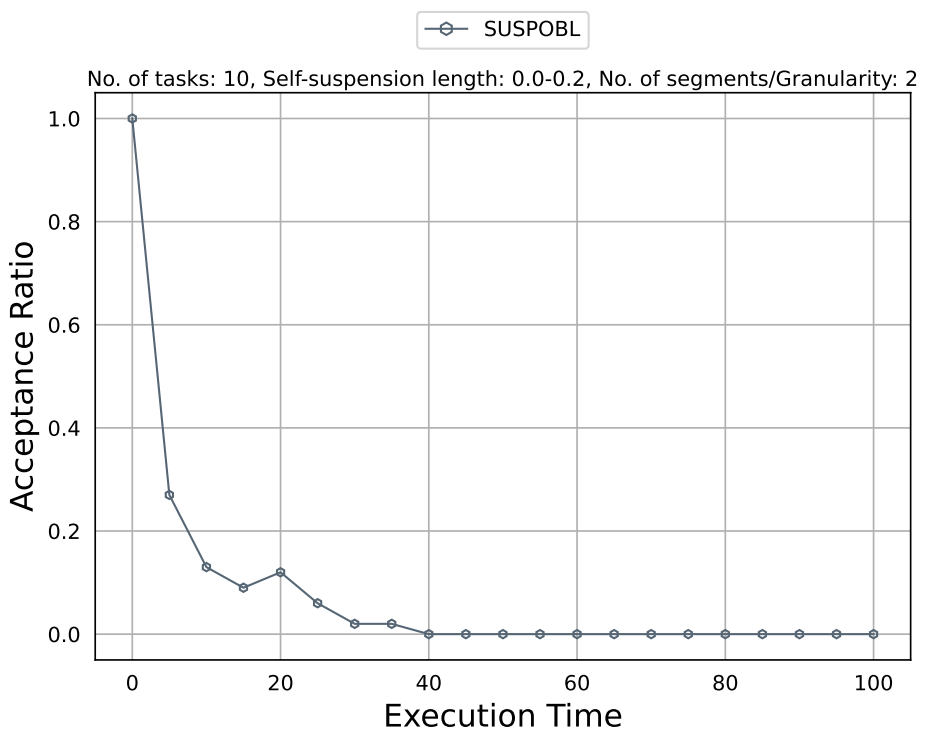
\includegraphics[width=\linewidth]{Capture.png}
		First UUnifast setup.

  
		\vspace{0.3cm}
		
		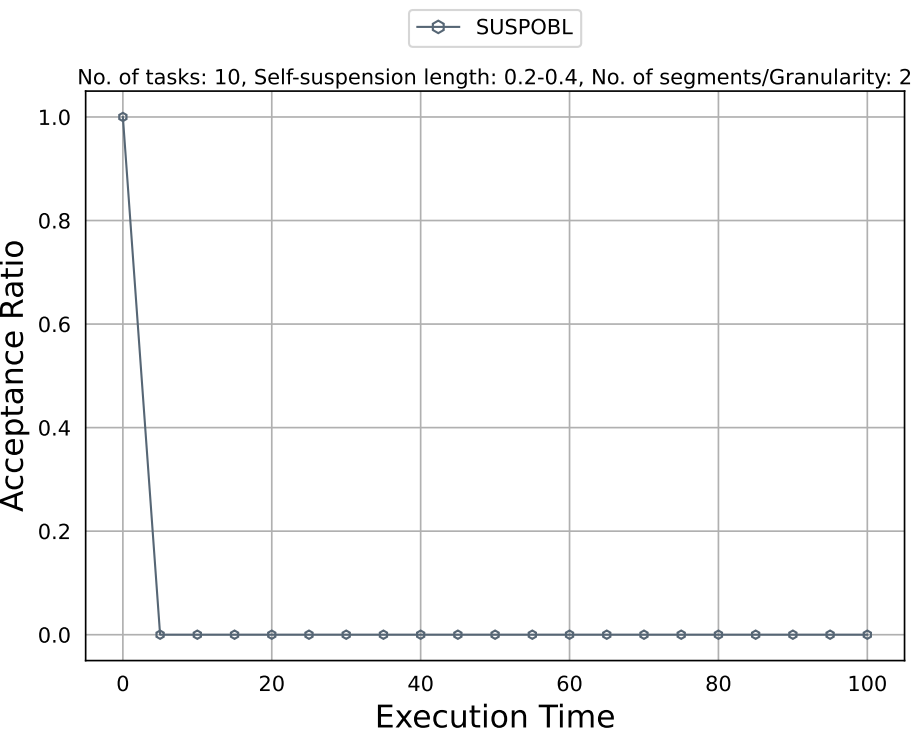
\includegraphics[width=\linewidth]{Capture2_uunifast.png}
		Second UUnifast setup.
		\vspace{0.3cm}
		
		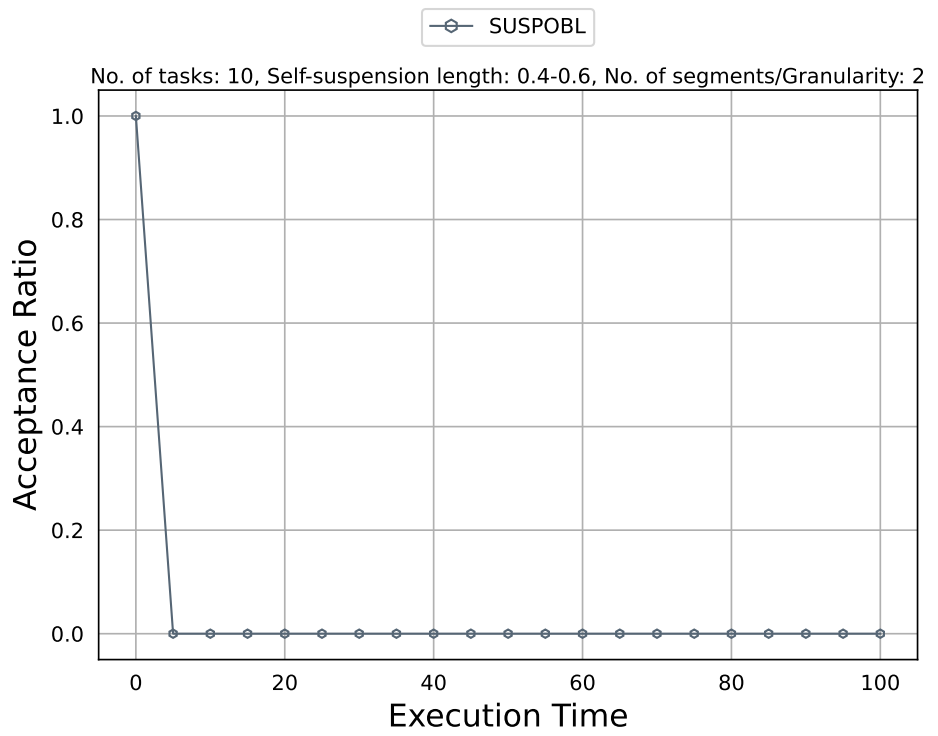
\includegraphics[width=\linewidth]{Capture3_uunifast.png}
		Third UUnifast setup.
		\vspace{0.3cm}
		
		
	\end{minipage}\hfill
	\begin{minipage}[t]{0.48\linewidth}
		\centering
		\textbf{(DRS)}
		\vspace{0.3cm}
		
		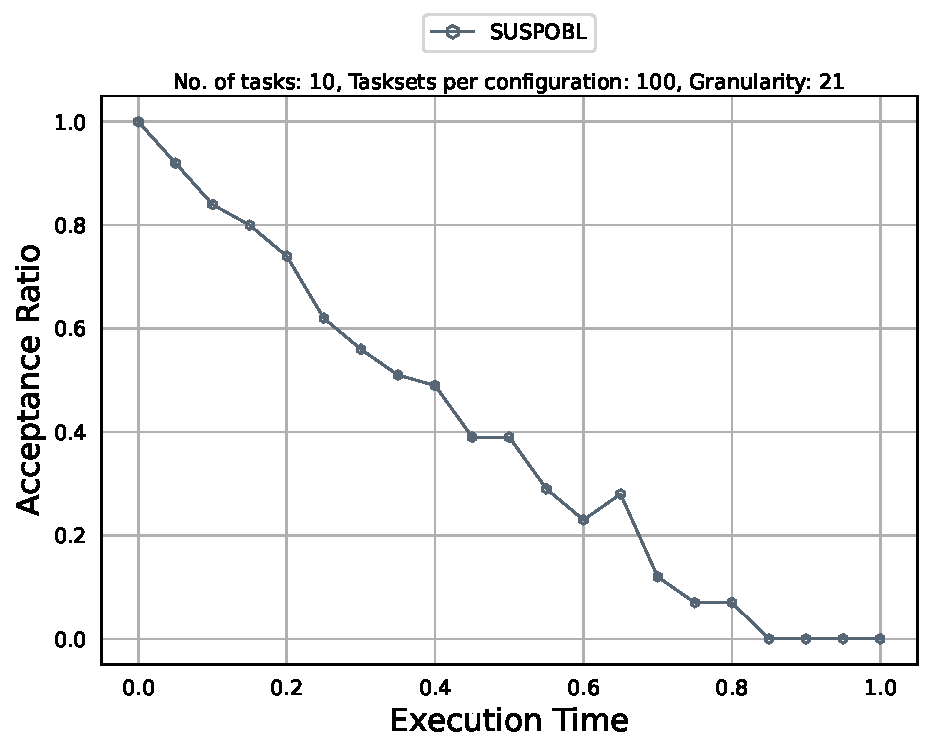
\includegraphics[width=\linewidth]{SUSPOBL_DRS_1stSetup.pdf}
		First DRS setup.
		\vspace{0.3cm}
		
		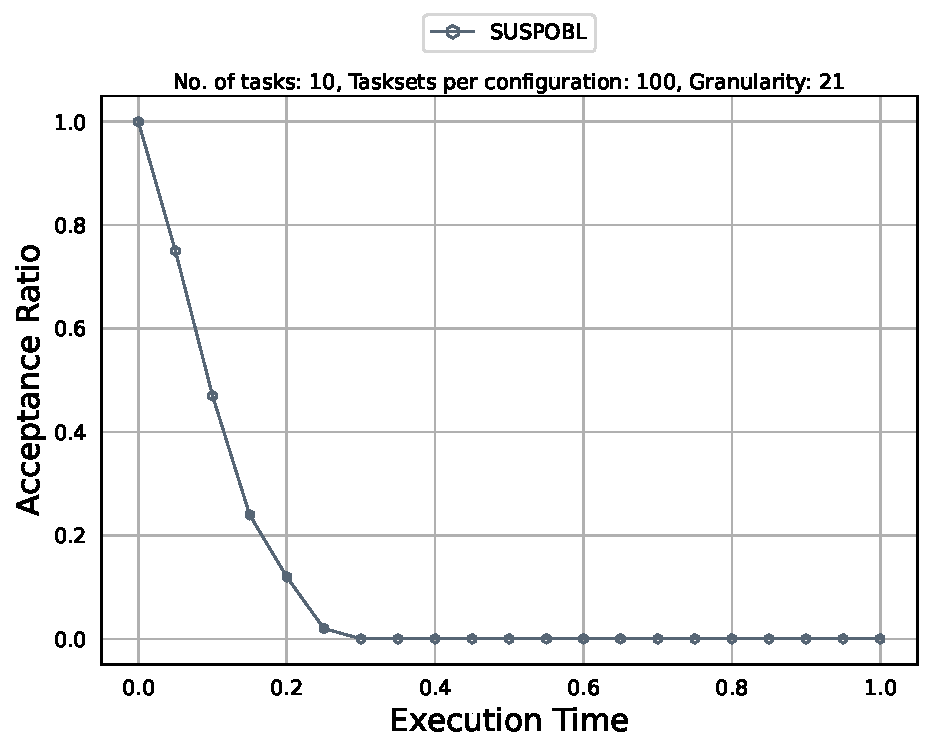
\includegraphics[width=\linewidth]{SUSPOBL_DRS_2ndSetup.pdf}
		Second DRS setup.
		\vspace{0.3cm}
		
		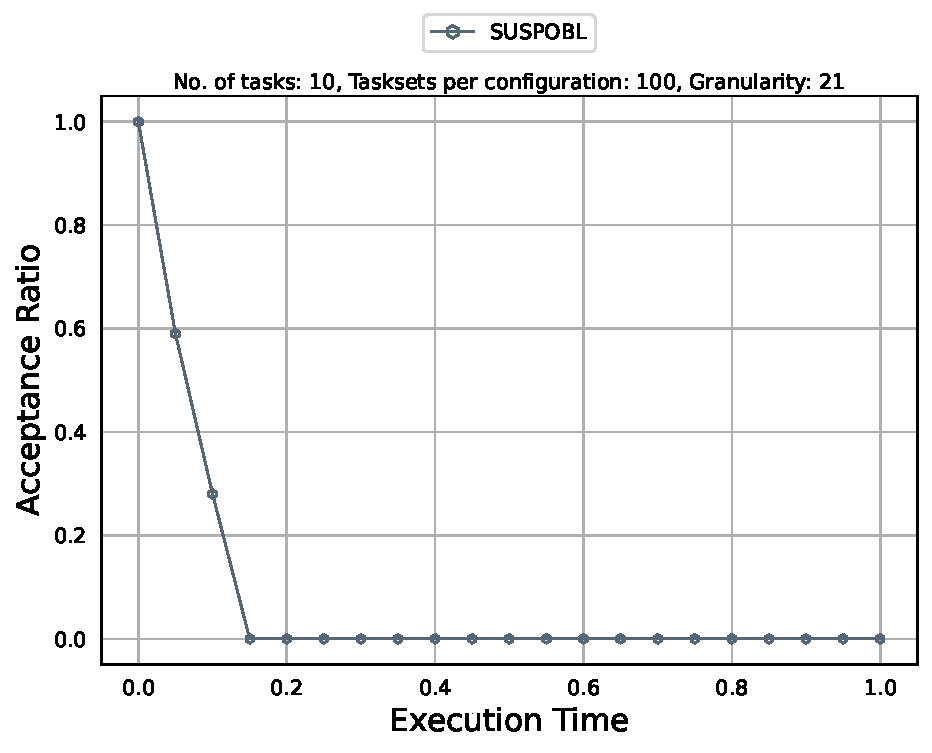
\includegraphics[width=\linewidth]{SUSPOBL_DRS_3rdSetup.pdf}
		Third DRS setup.
		\vspace{0.3cm}
	\end{minipage}

% ======================
	\clearpage
	\section{Suspension Jitter}
{
\raggedleft We are going to generate a suspension-jitter schedule for the DRS and UUniFast setups explained above \newline
}

	\begin{minipage}[t]{0.48\linewidth}
		\centering
		\textbf{(UUnifast)}
		\vspace{0.3cm}
		
		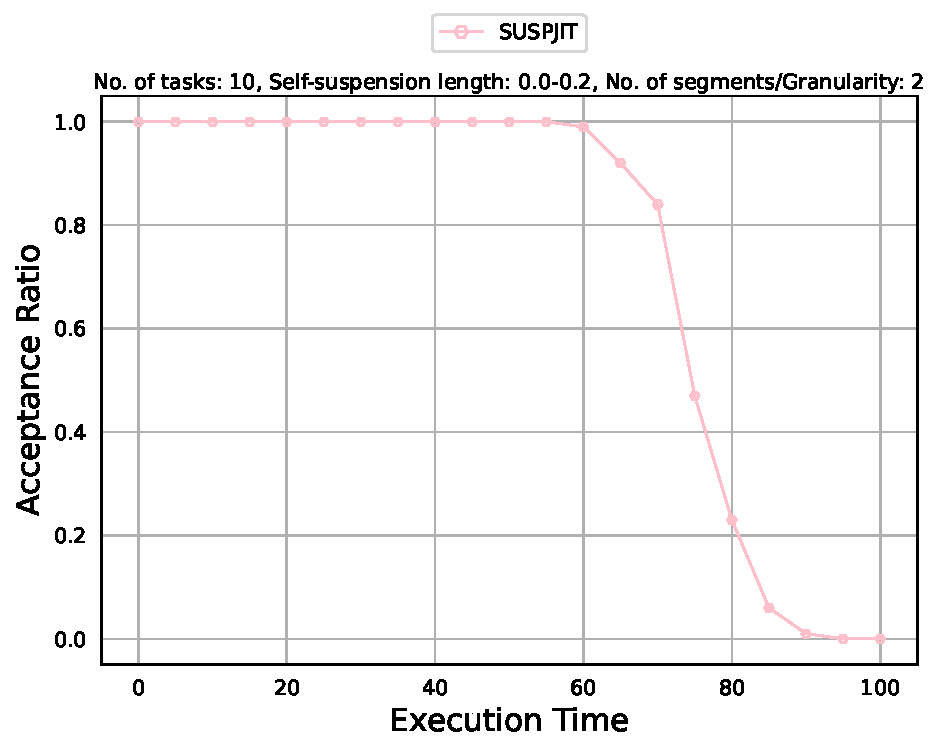
\includegraphics[width=\linewidth]{SUSPJIT[2][0.0-0.2][10].pdf}
		First UUnifast setup.
		\vspace{0.3cm}
		
		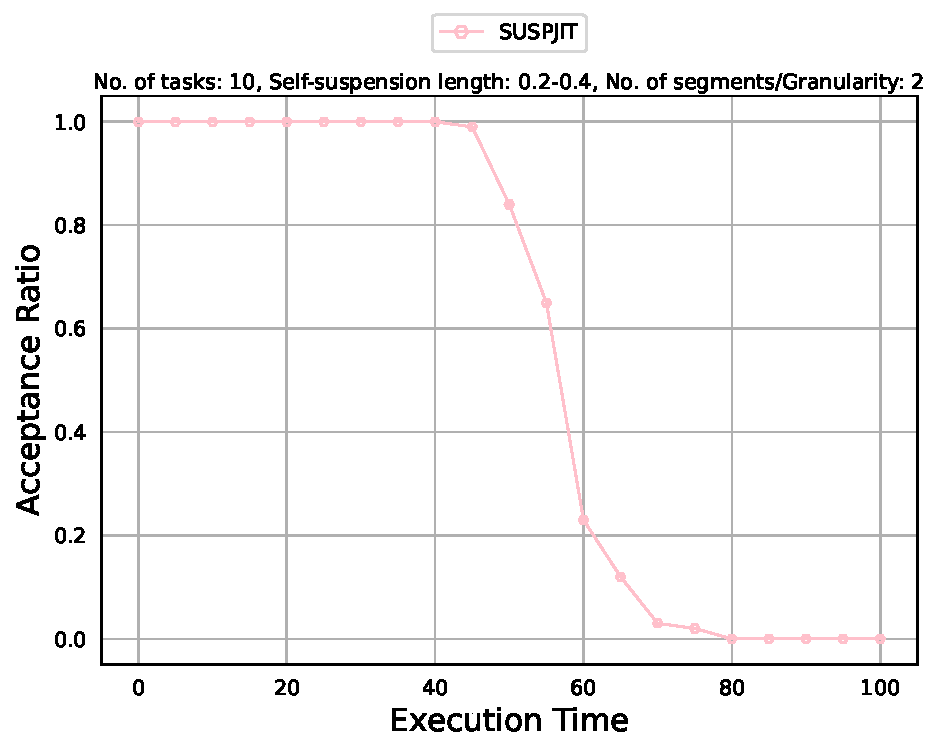
\includegraphics[width=\linewidth]{SUSPJIT[2][0.2-0.4][10].pdf}
		Second UUnifast setup.
		\vspace{0.3cm}
		
		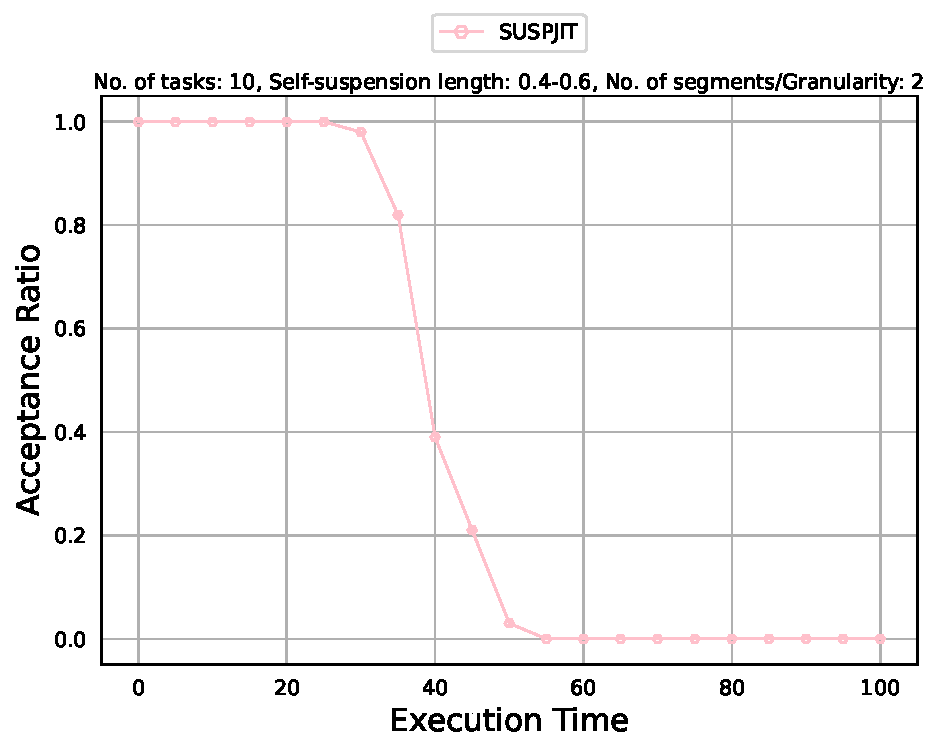
\includegraphics[width=\linewidth]{SUSPJIT[2][0.4-0.6][10].pdf}
		Third UUnifast setup.
		\vspace{0.3cm}
		
		
	\end{minipage}\hfill
	\begin{minipage}[t]{0.48\linewidth}
		\centering
		\textbf{(DRS)}
		\vspace{0.3cm}
		
		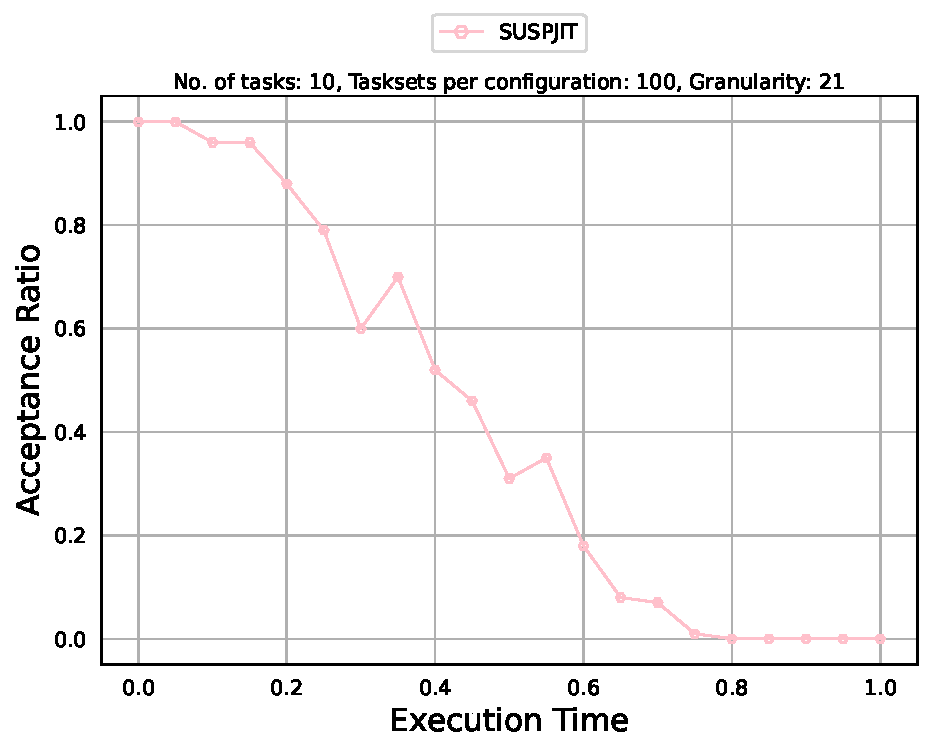
\includegraphics[width=\linewidth]{SUSPJIT_1stSetup.pdf}
		First DRS setup.
		\vspace{0.3cm}
		
		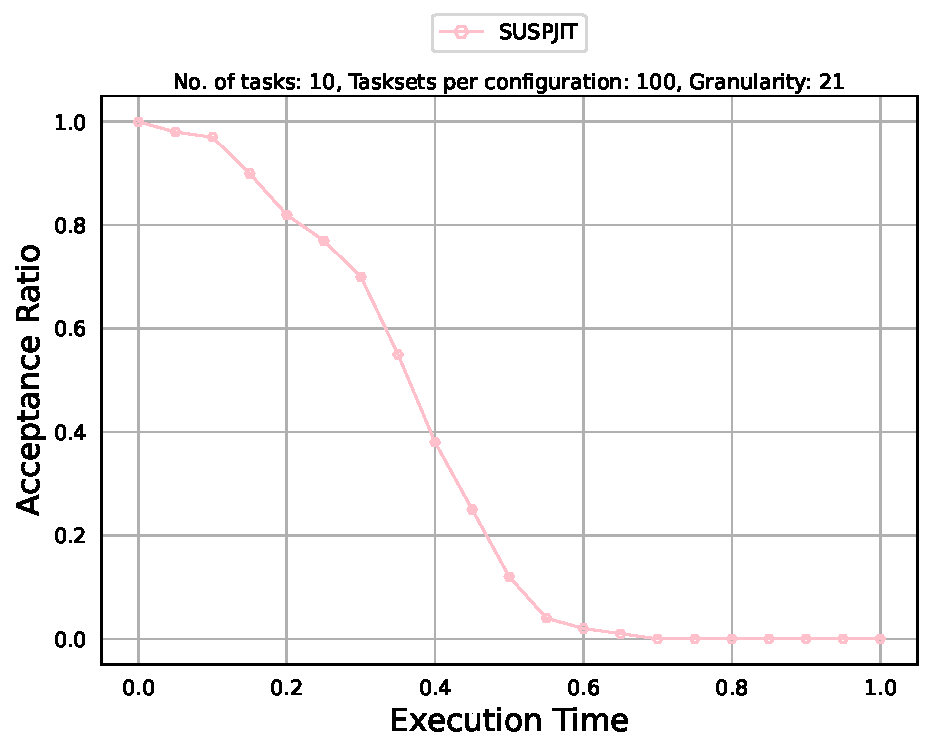
\includegraphics[width=\linewidth]{SUSPJIT_2ndSetup.pdf}
		Second DRS setup.
		\vspace{0.3cm}
		
		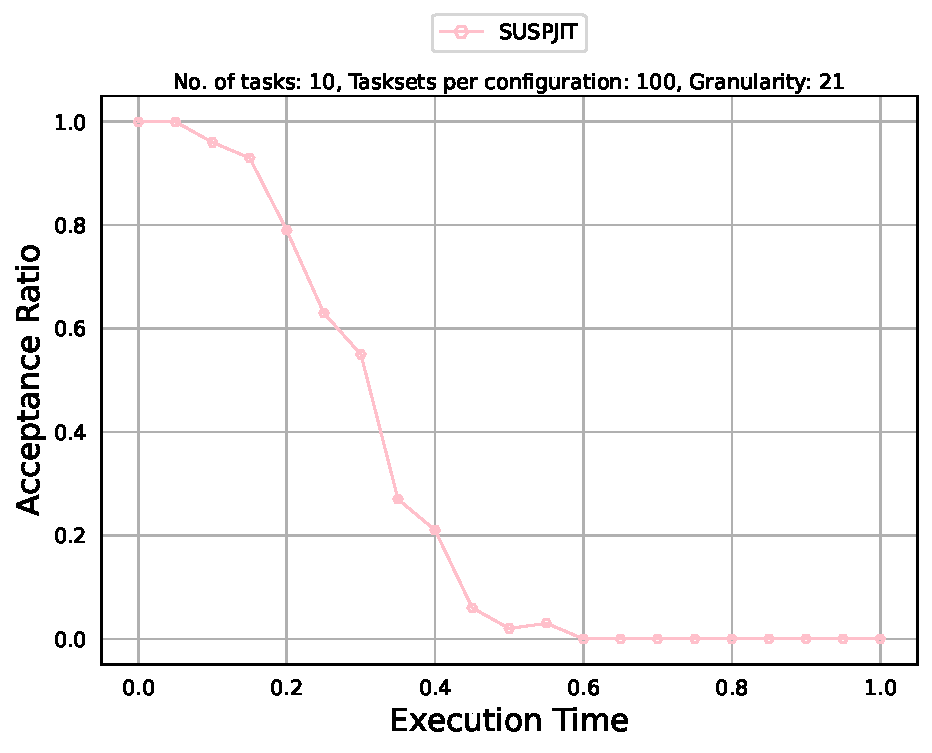
\includegraphics[width=\linewidth]{SUSPJIT_3rdSetup.pdf}
		Third DRS setup.
		\vspace{0.3cm}
	\end{minipage}

% ======================
	\clearpage
	\section{RSS}
{
\raggedleft We are going to generate a RSS schedule for the DRS and UUniFast setups explained above \newline
}

	\begin{minipage}[t]{0.48\linewidth}
		\centering
		\textbf{(UUnifast)}
		\vspace{0.3cm}
		
		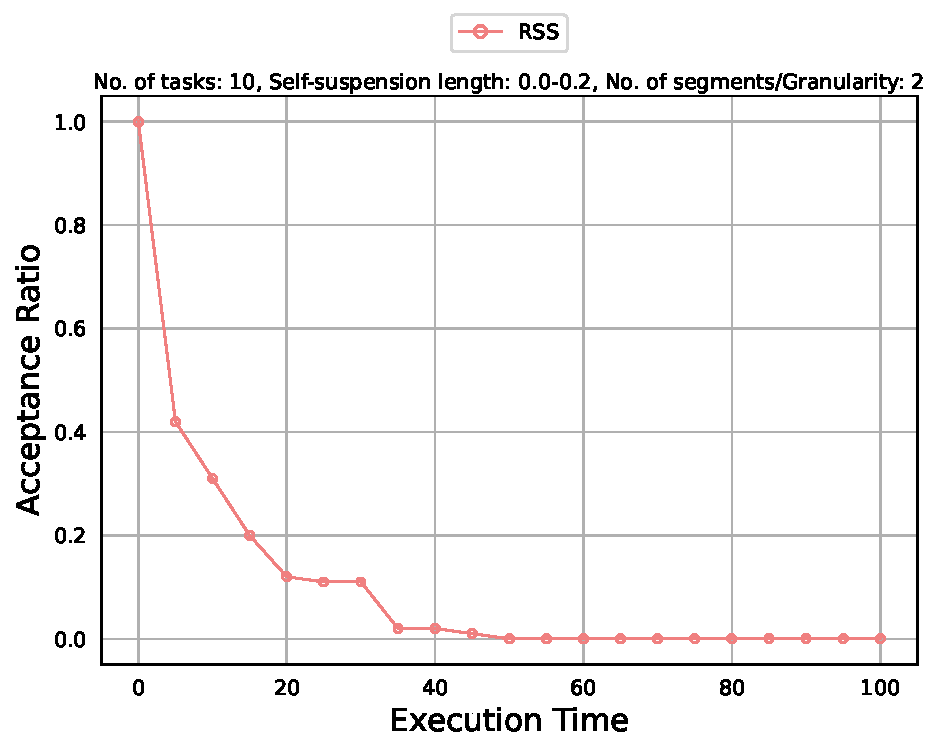
\includegraphics[width=\linewidth]{RSS[2][0.0-0.2][10].pdf}
		First UUnifast setup.
		\vspace{0.3cm}
		
		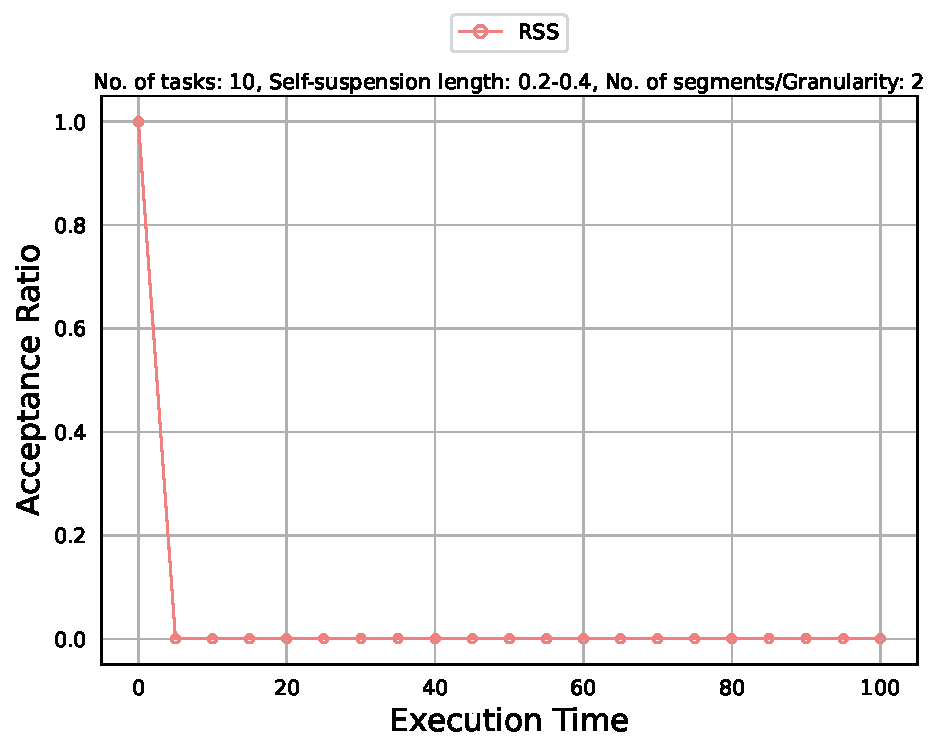
\includegraphics[width=\linewidth]{RSS[2][0.2-0.4][10].pdf}
		Second UUnifast setup.
		\vspace{0.3cm}
		
		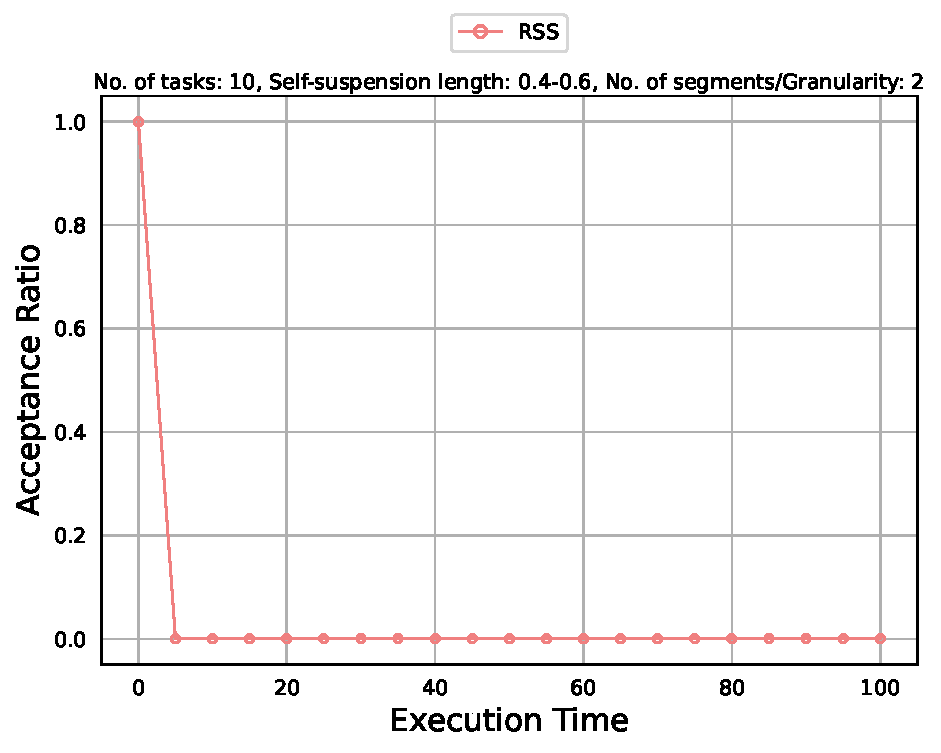
\includegraphics[width=\linewidth]{RSS[2][0.4-0.6][10].pdf}
		Third UUnifast setup.
		\vspace{0.3cm}
		
		
	\end{minipage}\hfill
	\begin{minipage}[t]{0.48\linewidth}
		\centering
		\textbf{(DRS)}
		\vspace{0.3cm}
		
		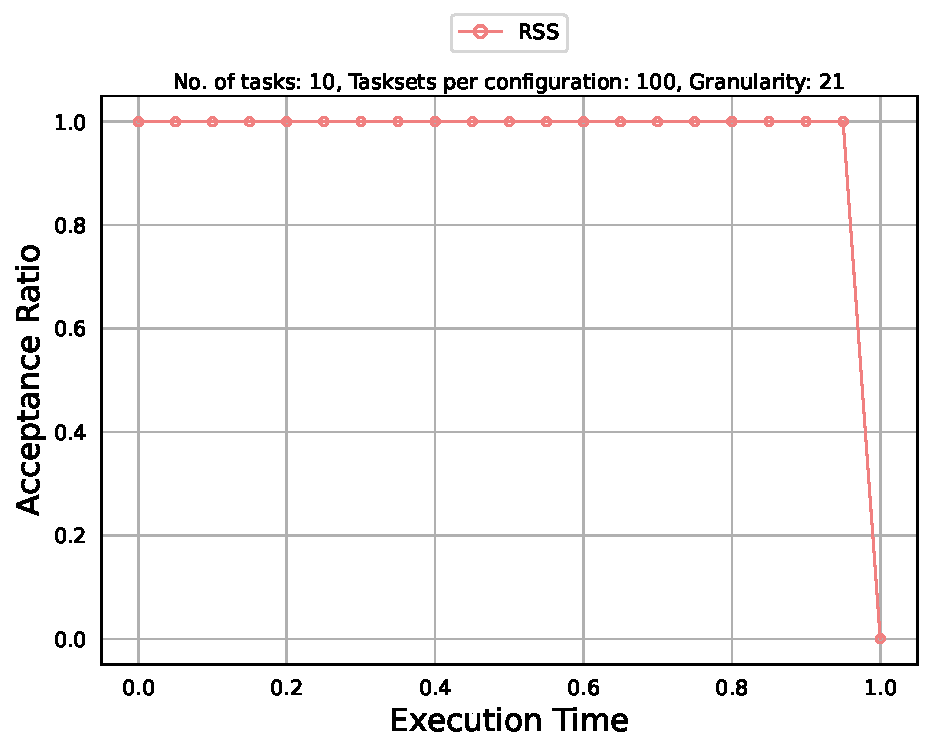
\includegraphics[width=\linewidth]{RSS_1stSetup_DRS.pdf}
		First DRS setup.
		\vspace{0.3cm}
		
		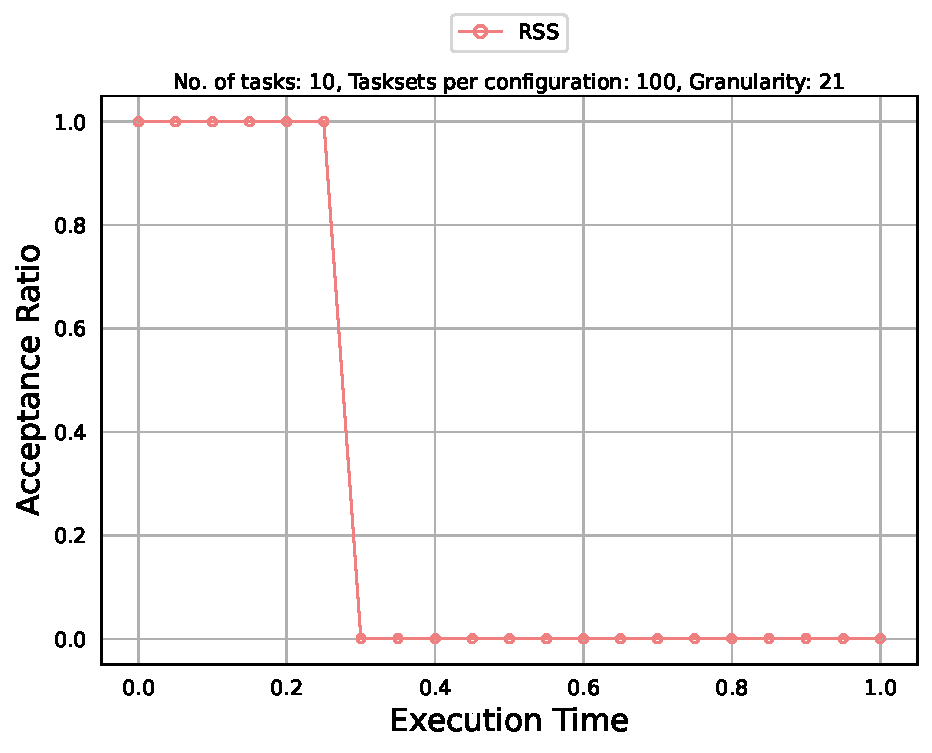
\includegraphics[width=\linewidth]{RSS_2ndSetup_DRS.pdf}
		Second DRS setup.
		\vspace{0.3cm}
		
		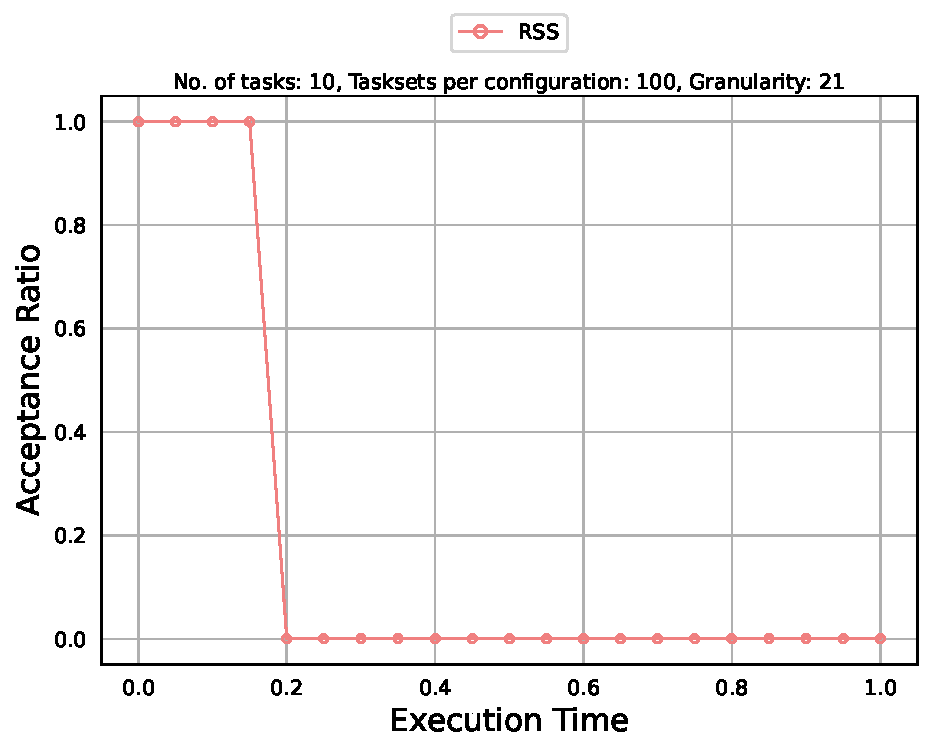
\includegraphics[width=\linewidth]{RSS_3rdSetup_DRS.pdf}
		Third DRS setup.
		\vspace{0.3cm}
	\end{minipage}

% ======================
	\clearpage
	\section{UDLEDF}
{
\raggedleft We are going to generate a UDLEDF schedule for the DRS and UUniFast setups explained above \newline
}

	\begin{minipage}[t]{0.48\linewidth}
		\centering
		\textbf{(UUnifast)}
		\vspace{0.3cm}
		
		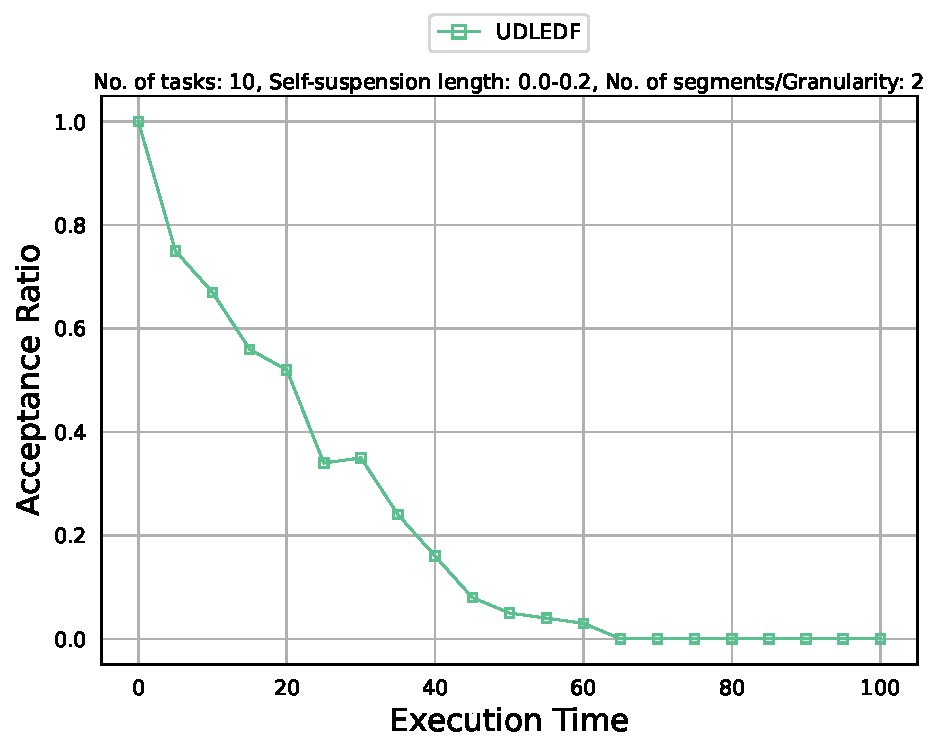
\includegraphics[width=\linewidth]{UDLEDF[2][0.0-0.2][10].pdf}
		First UUnifast setup.
		\vspace{0.3cm}
		
		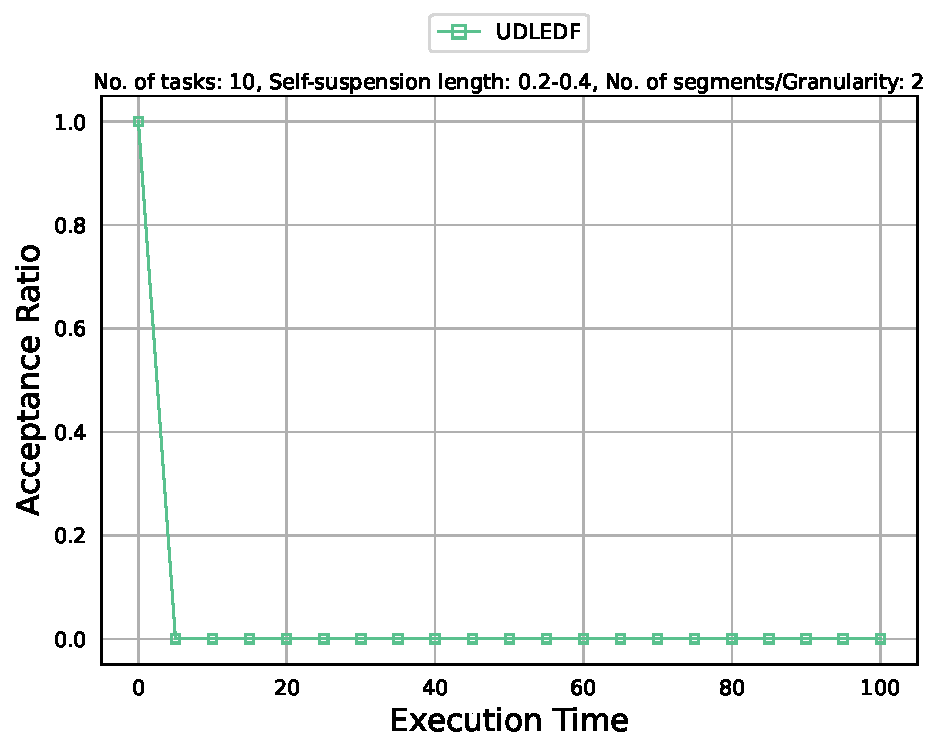
\includegraphics[width=\linewidth]{UDLEDF[2][0.2-0.4][10].pdf}
		Second UUnifast setup.
		\vspace{0.3cm}
		
		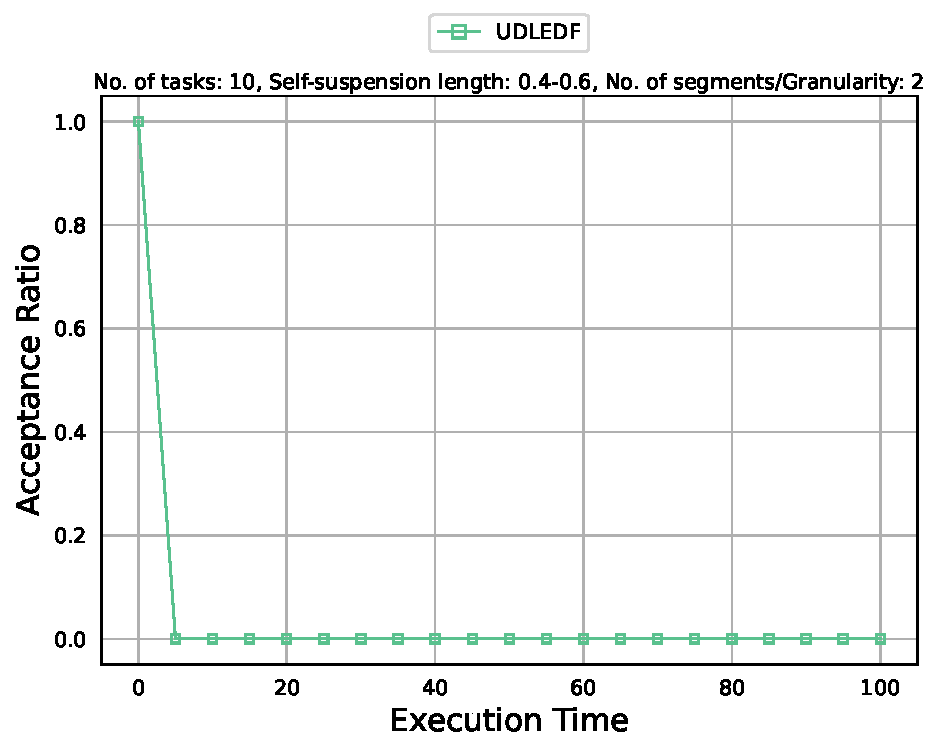
\includegraphics[width=\linewidth]{UDLEDF[2][0.4-0.6][10].pdf}
		Third UUnifast setup.
		\vspace{0.3cm}
		
		
	\end{minipage}\hfill
	\begin{minipage}[t]{0.48\linewidth}
		\centering
		\textbf{(DRS)}
		\vspace{0.3cm}
		
		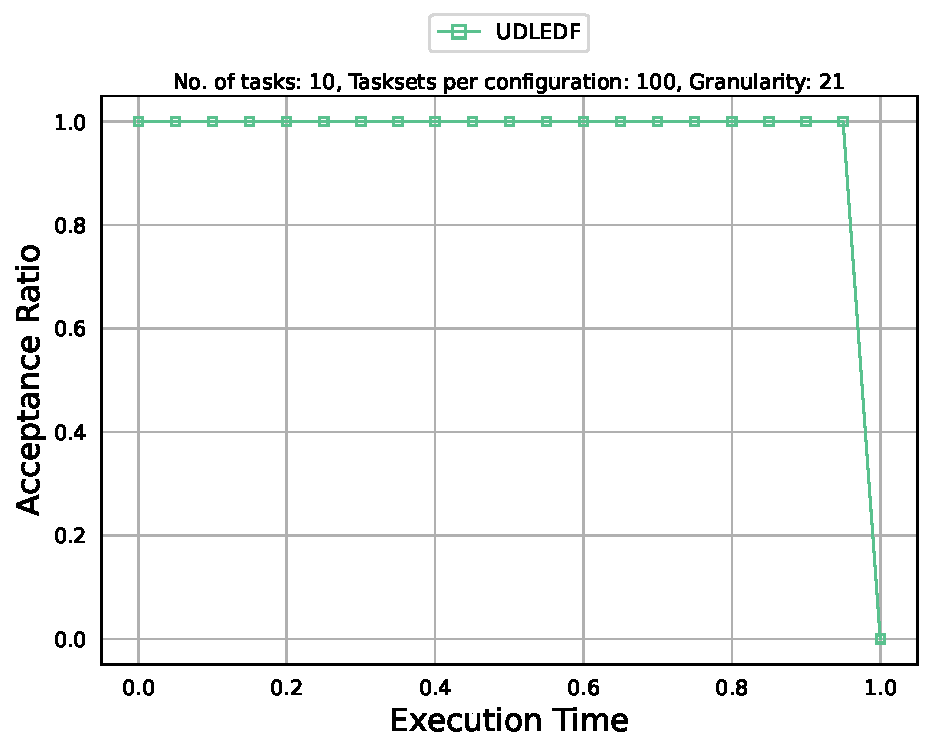
\includegraphics[width=\linewidth]{UDLEDF_1stSetup_DRS.pdf}
		First DRS setup.
		\vspace{0.3cm}
		
		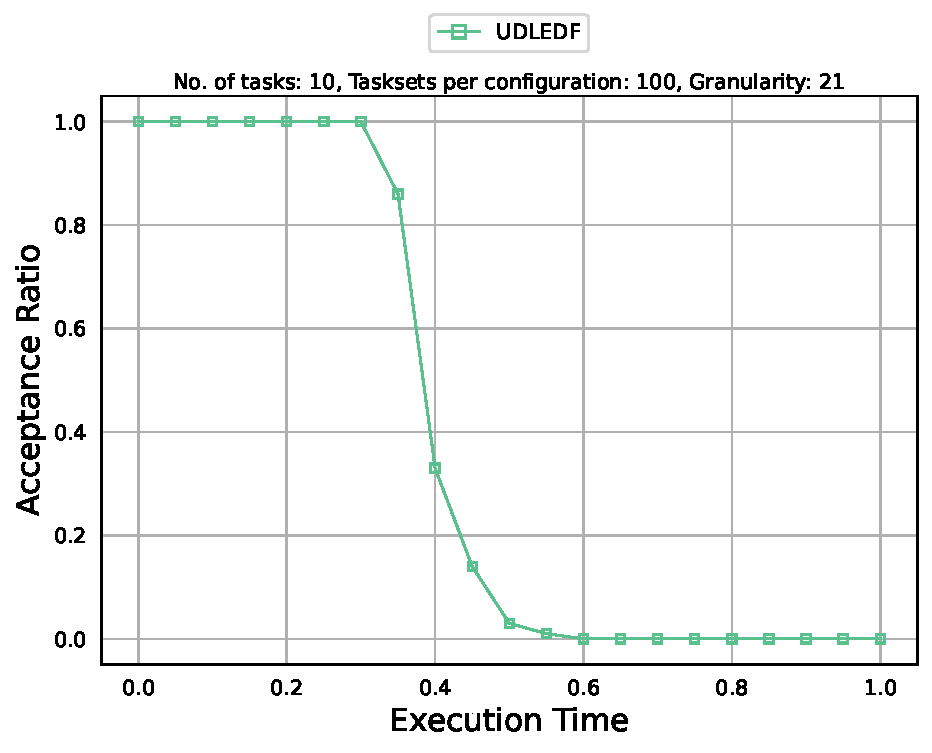
\includegraphics[width=\linewidth]{UDLEDF_2ndSetup_DRS.pdf}
		Second DRS setup.
		\vspace{0.3cm}
		
		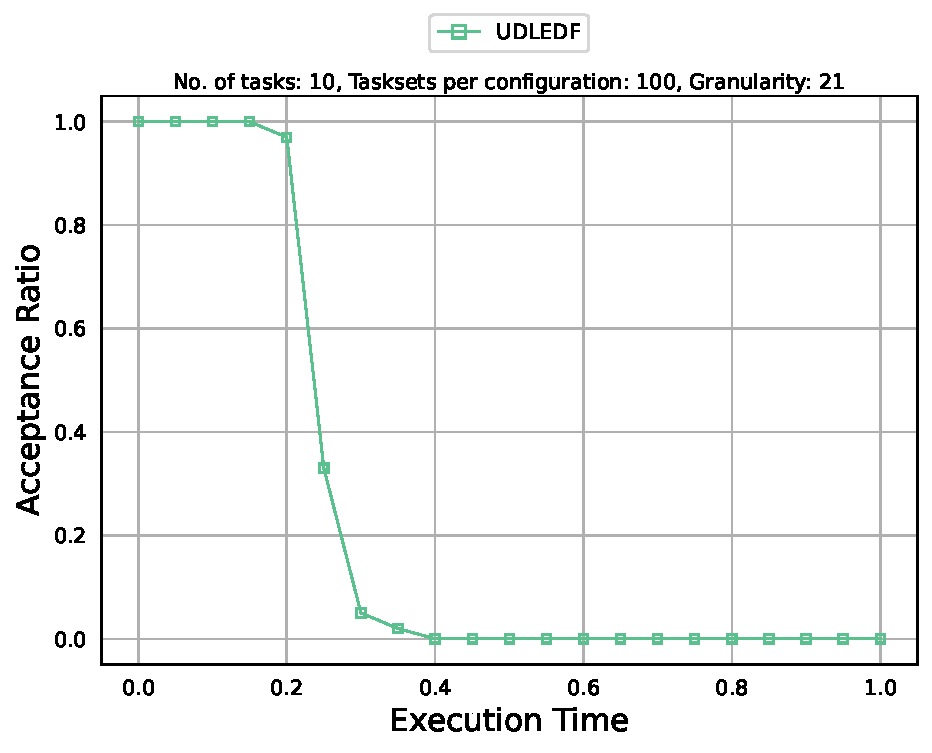
\includegraphics[width=\linewidth]{UDLEDF_3rdSetup_DRS.pdf}
		Third DRS setup.
		\vspace{0.3cm}
	\end{minipage}


% ======================
	\clearpage
	\section{WLAEDF}
{
\raggedleft We are going to generate a WLAEDF schedule for the DRS and UUniFast setups explained above \newline
}

	\begin{minipage}[t]{0.48\linewidth}
		\centering
		\textbf{(UUnifast)}
		\vspace{0.3cm}
		
		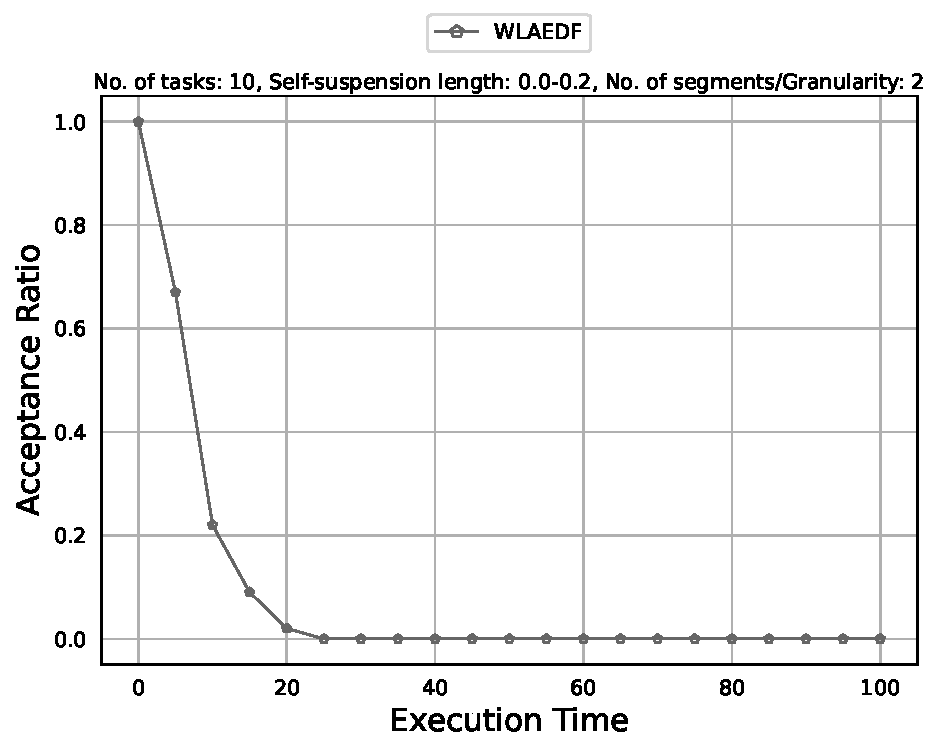
\includegraphics[width=\linewidth]{WLAEDF[2][0.0-0.2][10].pdf}
		First UUnifast setup.
		\vspace{0.3cm}
		
		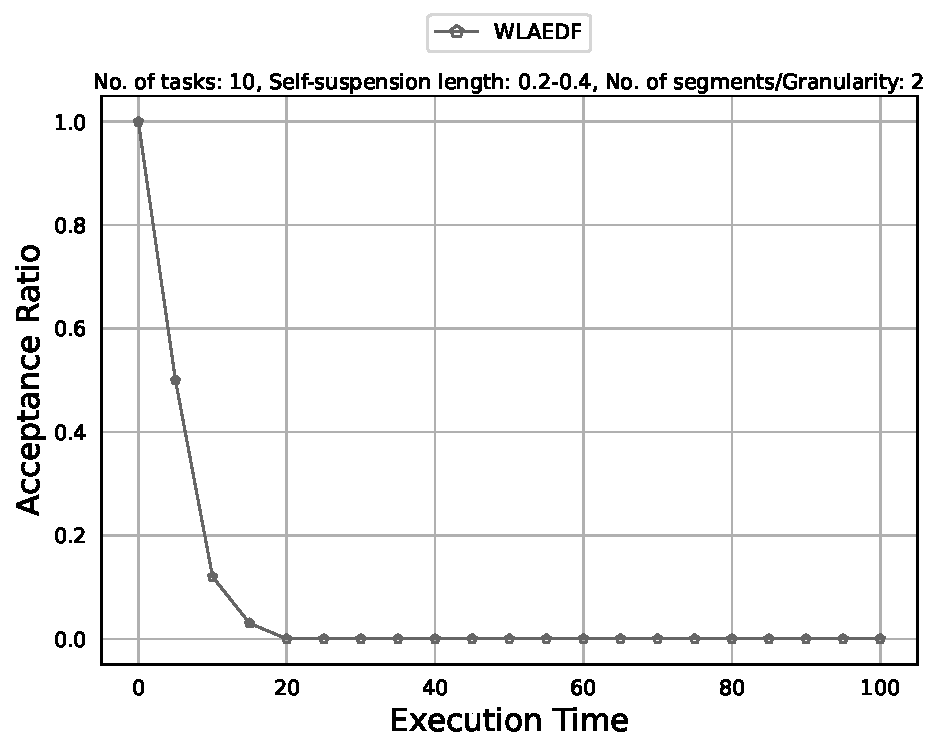
\includegraphics[width=\linewidth]{WLAEDF[2][0.2-0.4][10].pdf}
		Second UUnifast setup.
		\vspace{0.3cm}
		
		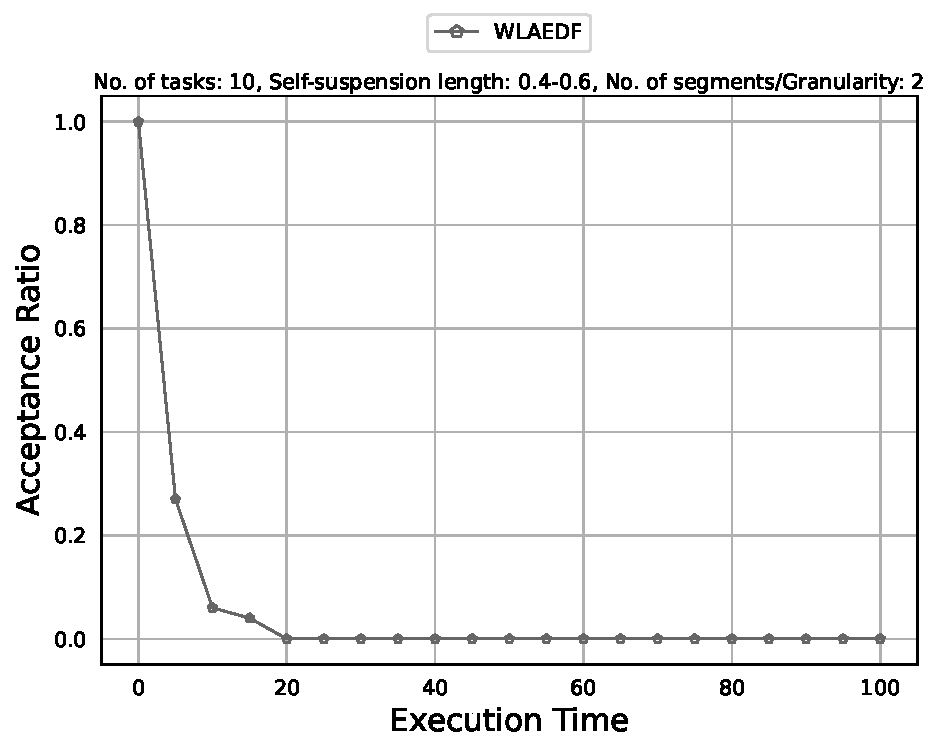
\includegraphics[width=\linewidth]{WLAEDF[2][0.4-0.6][10].pdf}
		Third UUnifast setup.
		\vspace{0.3cm}
		
		
	\end{minipage}\hfill
	\begin{minipage}[t]{0.48\linewidth}
		\centering
		\textbf{(DRS)}
		\vspace{0.3cm}
		
		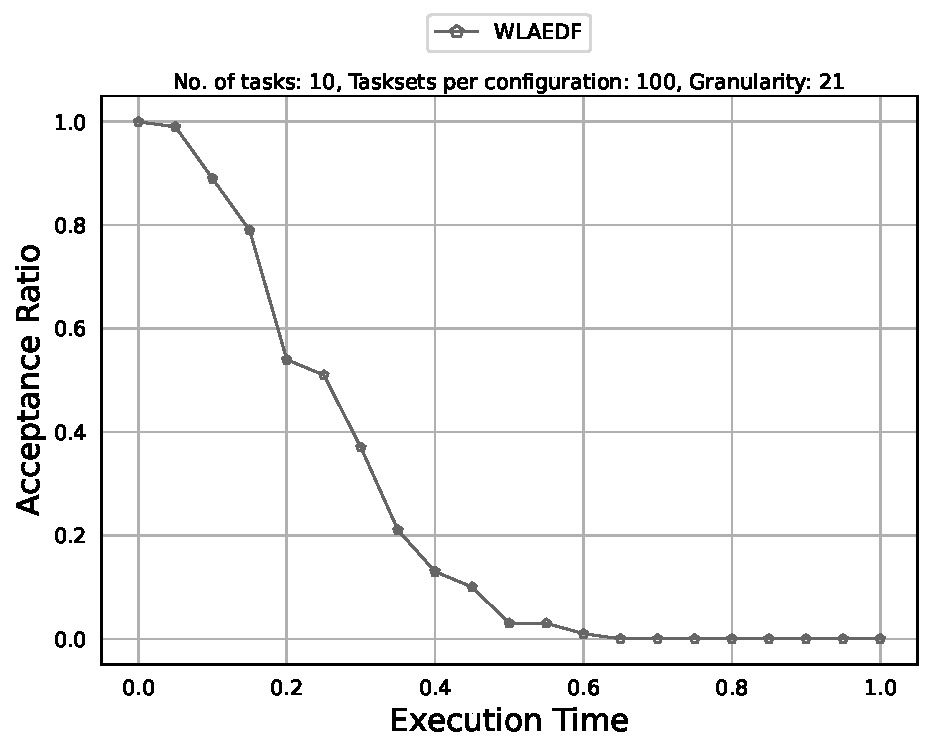
\includegraphics[width=\linewidth]{WLAEDF_1stSetup_DRS.pdf}
		First DRS setup.
		\vspace{0.3cm}
		
		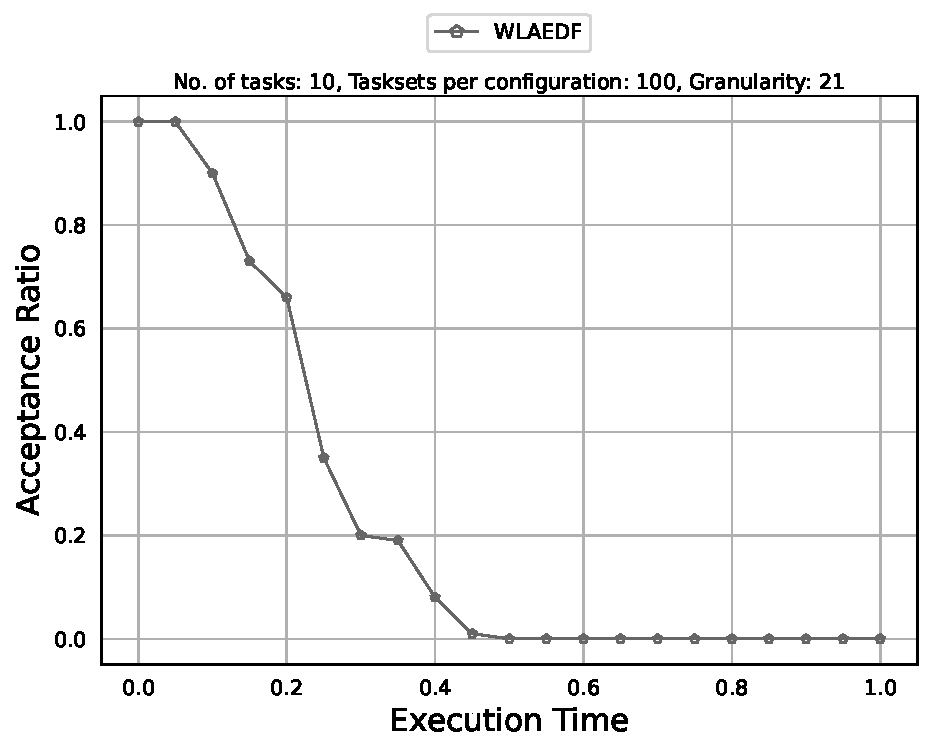
\includegraphics[width=\linewidth]{WLAEDF_2ndSetup_DRS.pdf}
		Second DRS setup.
		\vspace{0.3cm}
		
		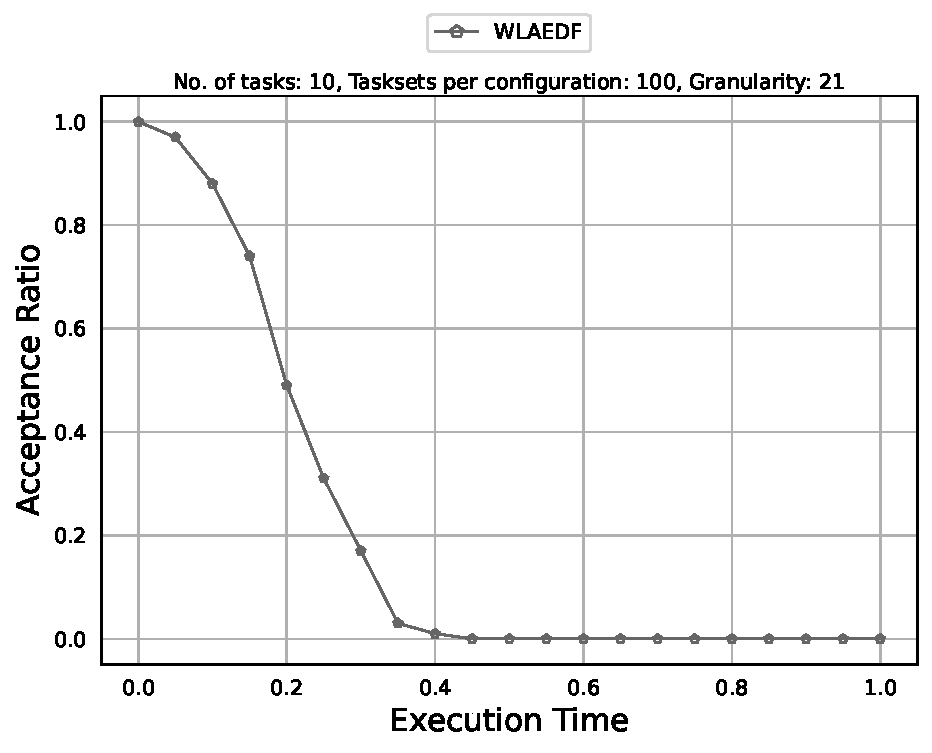
\includegraphics[width=\linewidth]{WLAEDF_3rdSetup_DRS.pdf}
		Third DRS setup.
		\vspace{0.3cm}
	\end{minipage}


% ======================
	\clearpage
	\section{RTEDF}
{
\raggedleft We are going to generate a RTEDF schedule for the DRS and UUniFast setups explained above \newline
}

	\begin{minipage}[t]{0.48\linewidth}
		\centering
		\textbf{(UUnifast)}
		\vspace{0.3cm}
		
		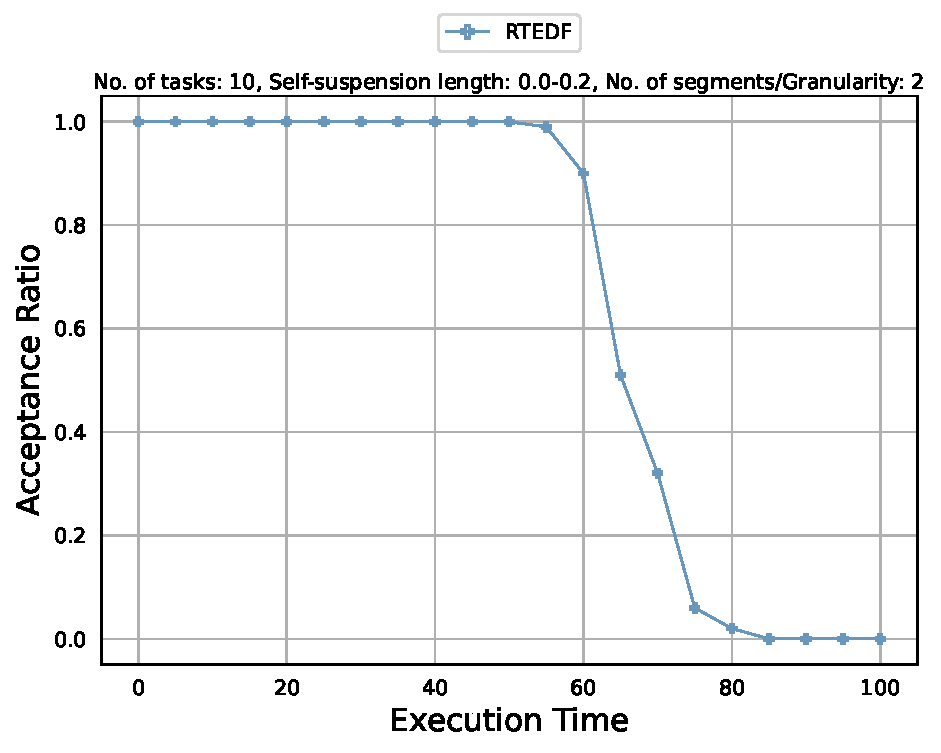
\includegraphics[width=\linewidth]{RTEDF[2][0.0-0.2][10].pdf}
		First UUnifast setup.
		\vspace{0.3cm}
		
		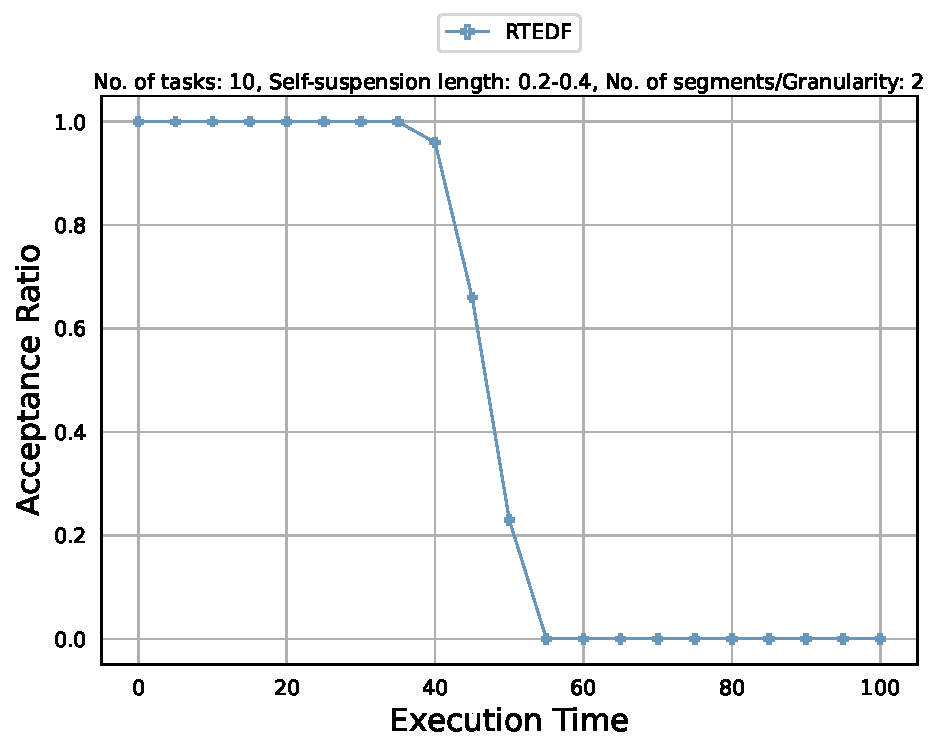
\includegraphics[width=\linewidth]{RTEDF[2][0.2-0.4][10].pdf}
		Second UUnifast setup.
		\vspace{0.3cm}
		
		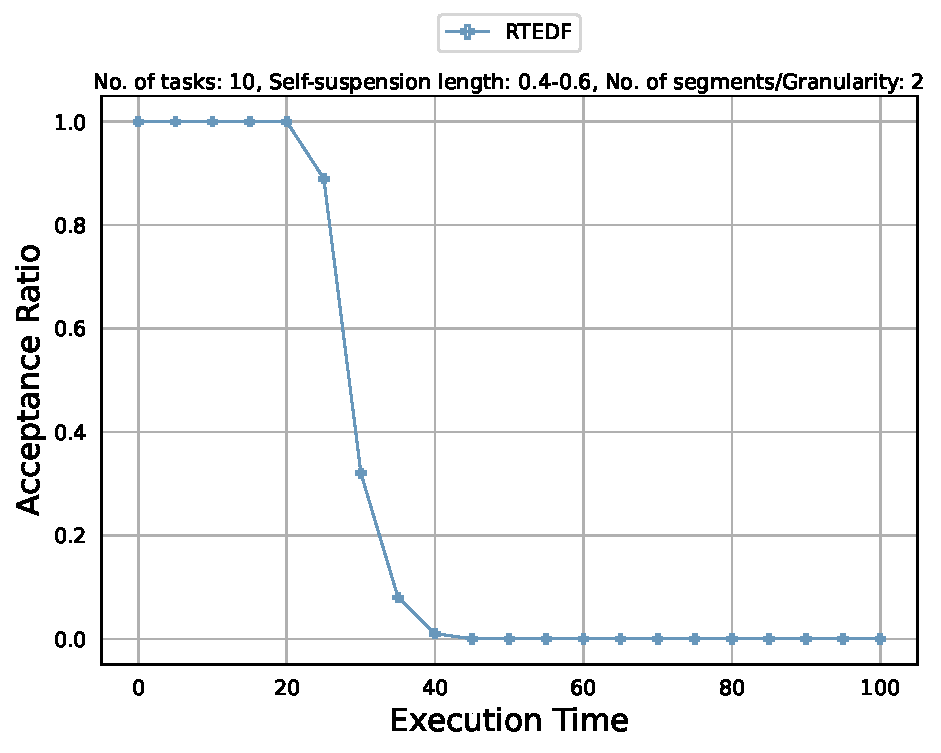
\includegraphics[width=\linewidth]{RTEDF[2][0.4-0.6][10].pdf}
		Third UUnifast setup.
		\vspace{0.3cm}
		
		
	\end{minipage}\hfill
	\begin{minipage}[t]{0.48\linewidth}
		\centering
		\textbf{(DRS)}
		\vspace{0.3cm}
		
		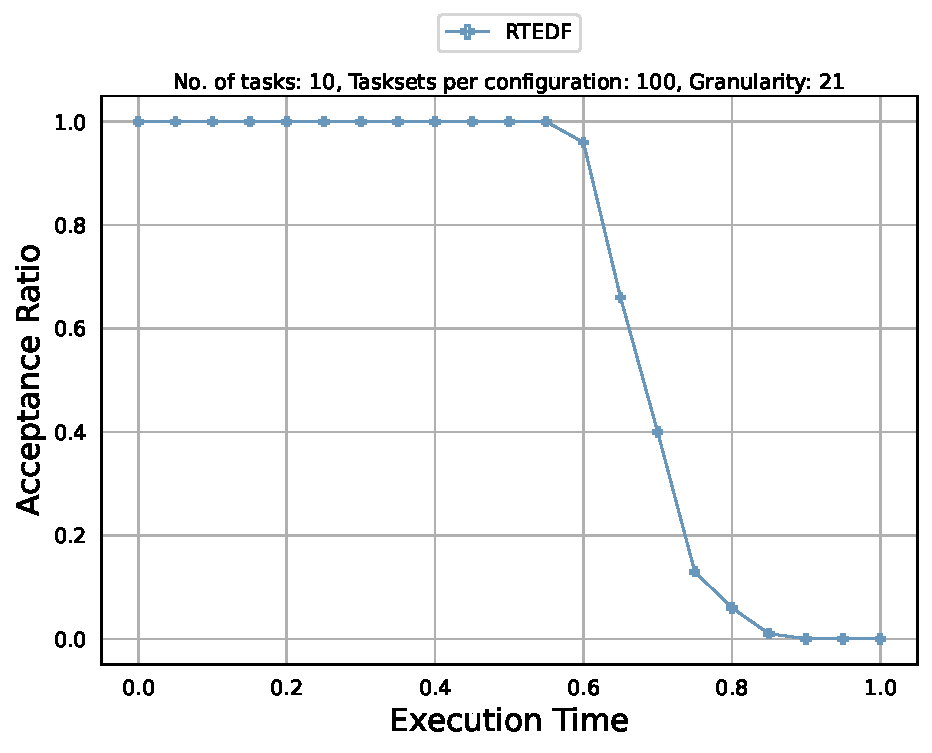
\includegraphics[width=\linewidth]{RTEDF_1stSetup_DRS.pdf}
		First DRS setup.
		\vspace{0.3cm}
		
		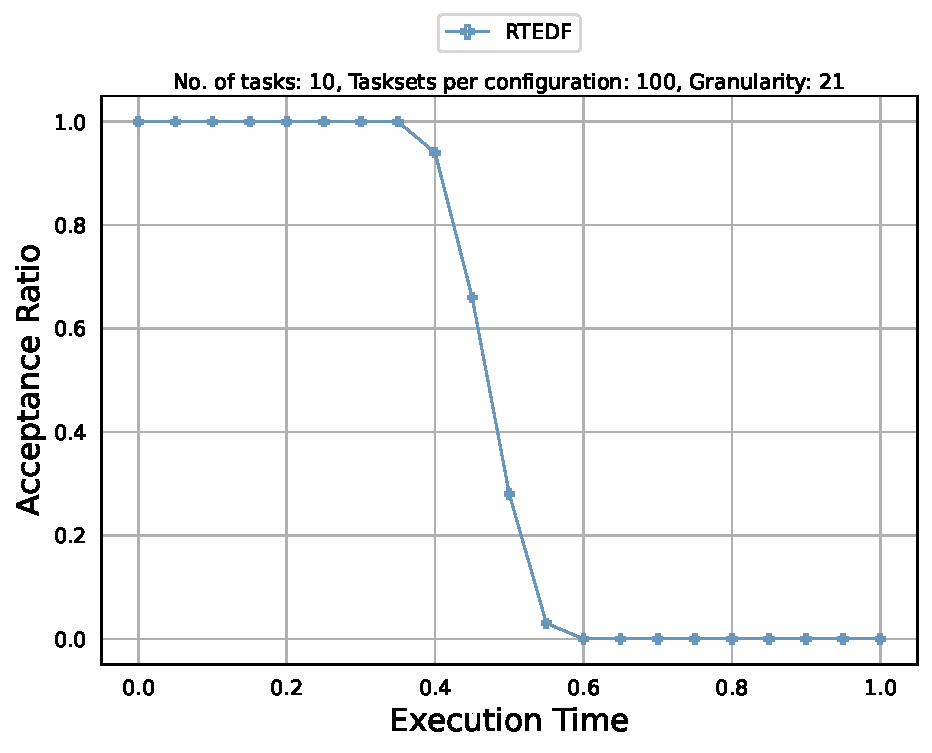
\includegraphics[width=\linewidth]{RTEDF_2ndSetup_DRS.pdf}
		Second DRS setup.
		\vspace{0.3cm}
		
		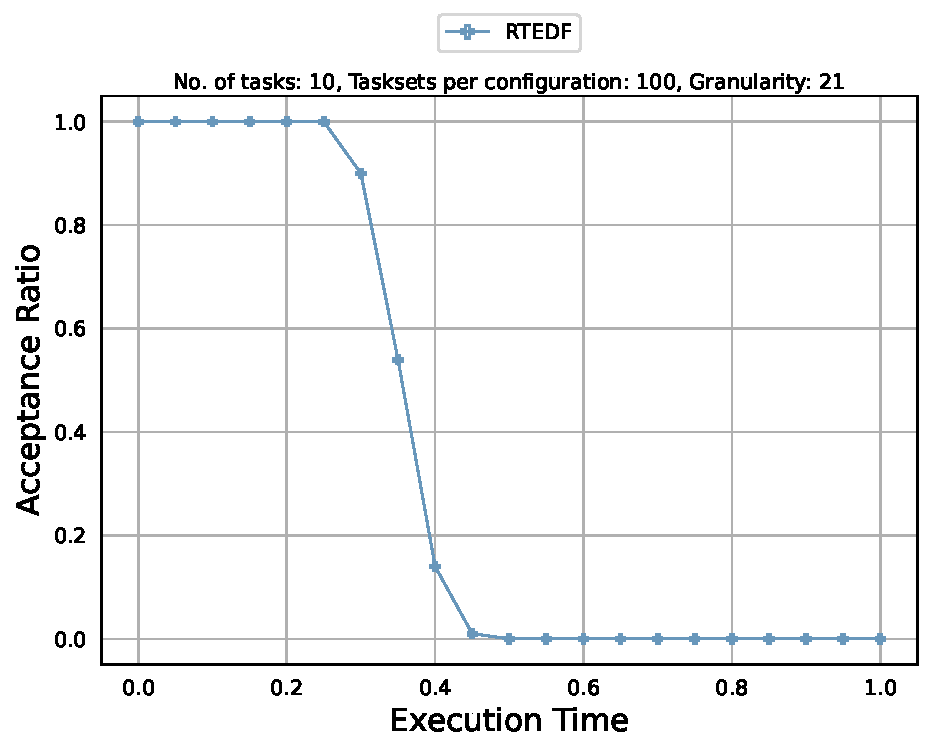
\includegraphics[width=\linewidth]{RTEDF_3rdSetup_DRS.pdf}
		Third DRS setup.
		\vspace{0.3cm}
	\end{minipage}


% ======================
	\clearpage
	\section{UNIFRAMEWORK}
{
\raggedleft We are going to generate a Uniframework schedule for the DRS and UUniFast setups explained above \newline
}

	\begin{minipage}[t]{0.48\linewidth}
		\centering
		\textbf{(UUnifast)}
		\vspace{0.3cm}
		
		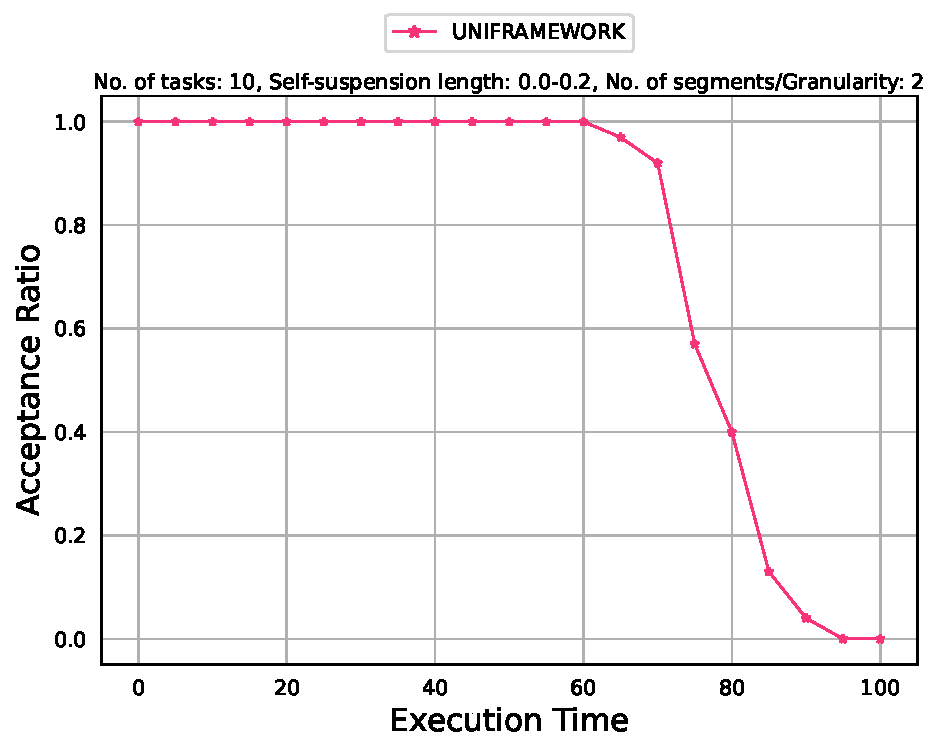
\includegraphics[width=\linewidth]{UNIFRAMEWORK[2][0.0-0.2][10].pdf}
		First UUnifast setup.
		\vspace{0.3cm}
		
		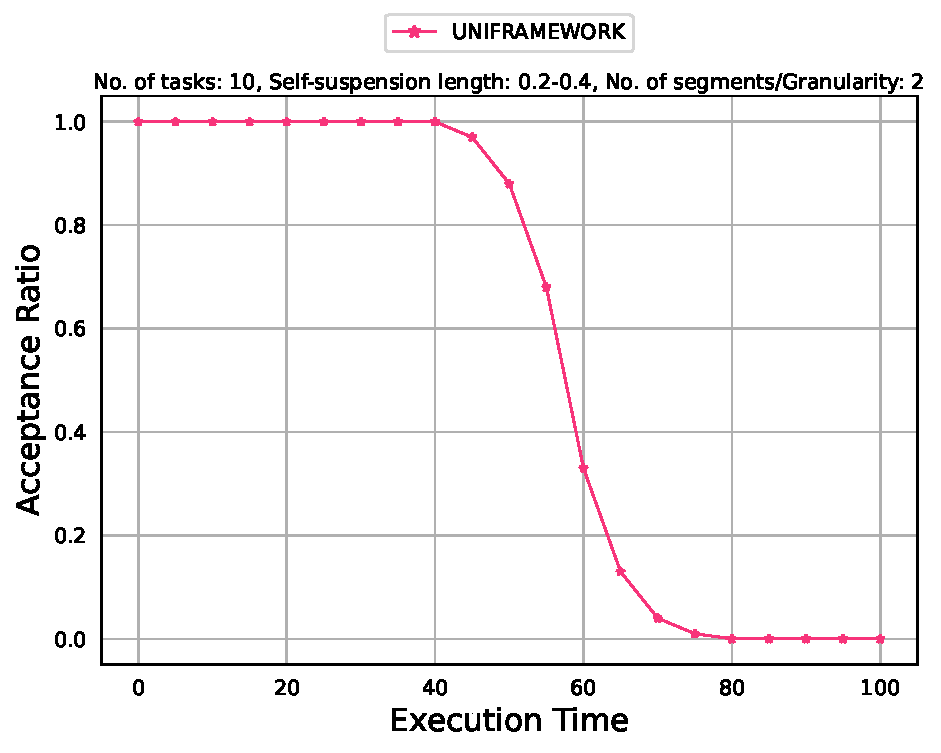
\includegraphics[width=\linewidth]{UNIFRAMEWORK[2][0.2-0.4][10].pdf}
		Second UUnifast setup.
		\vspace{0.3cm}
		
		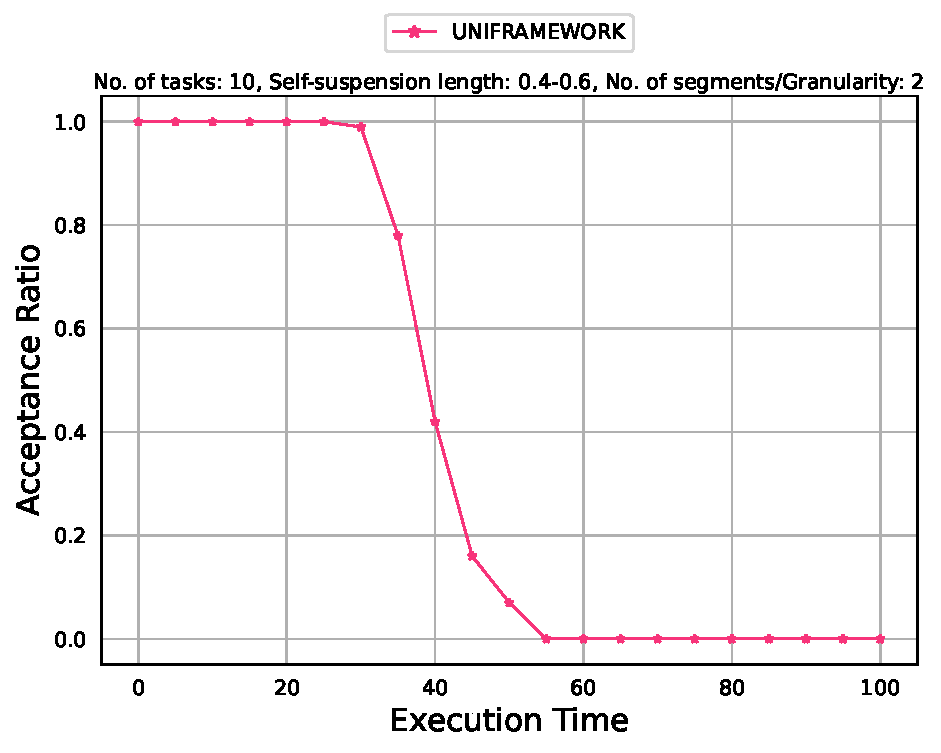
\includegraphics[width=\linewidth]{UNIFRAMEWORK[2][0.4-0.6][10].pdf}
		Third UUnifast setup.
		\vspace{0.3cm}
		
		
	\end{minipage}\hfill
	\begin{minipage}[t]{0.48\linewidth}
		\centering
		\textbf{(DRS)}
		\vspace{0.3cm}
		
		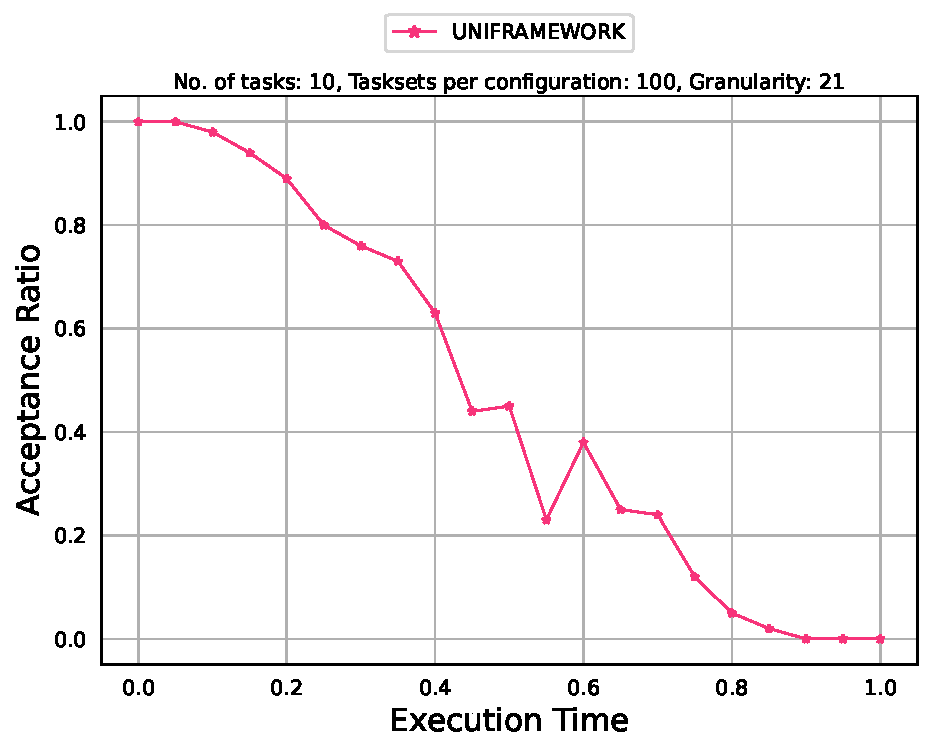
\includegraphics[width=\linewidth]{UNIFRAMEWORK_1stSetup_DRS.pdf}
		First DRS setup.
		\vspace{0.3cm}
		
		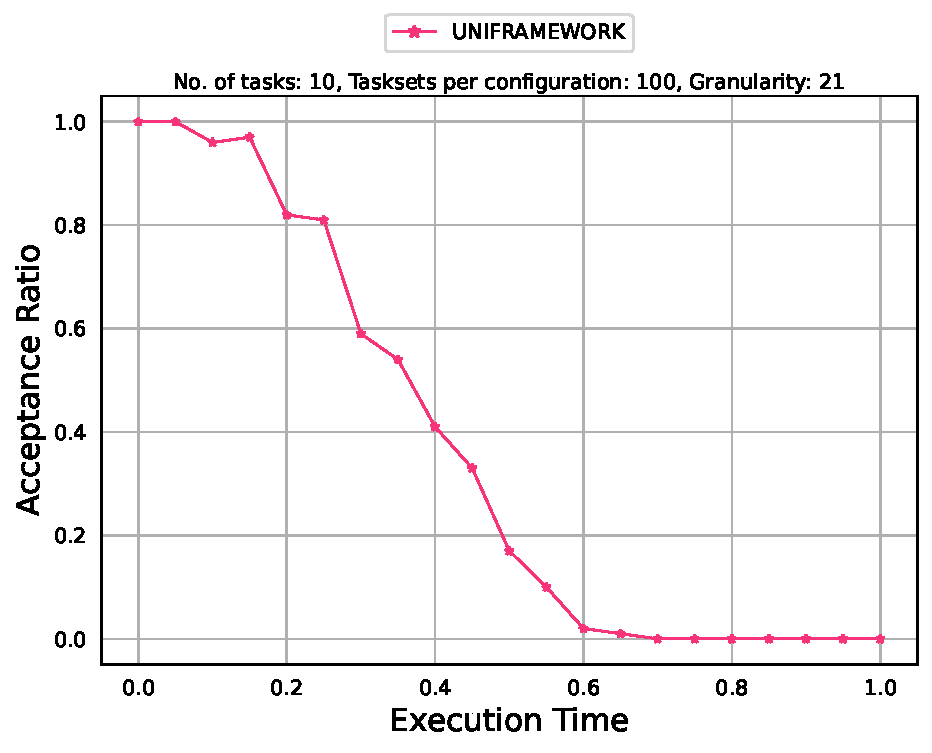
\includegraphics[width=\linewidth]{UNIFRAMEWORK_2ndSetup_DRS.pdf}
		Second DRS setup.
		\vspace{0.3cm}
		
		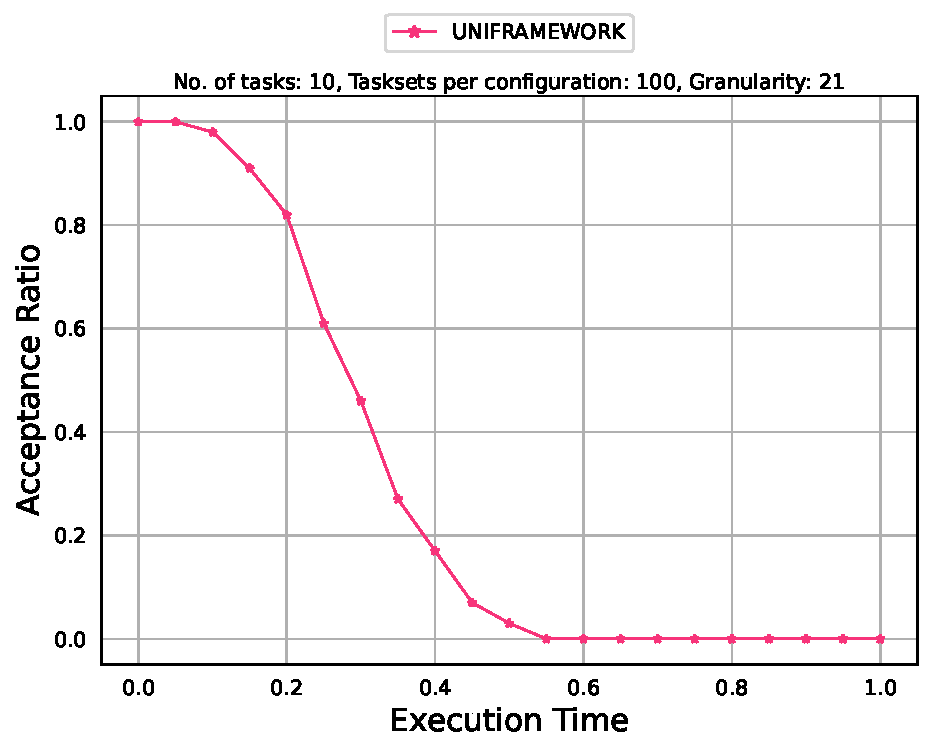
\includegraphics[width=\linewidth]{UNIFRAMEWORK_3rdSetup_DRS.pdf}
		Third DRS setup.
		\vspace{0.3cm}
	\end{minipage}


% ======================
	\clearpage
	\section{Suspension Block}
{
\raggedleft We are going to generate a Suspension Block schedule for the DRS and UUniFast setups explained above \newline 
}

	\begin{minipage}[t]{0.48\linewidth}
		\centering
		\textbf{(UUnifast)}
		\vspace{0.3cm}
		
		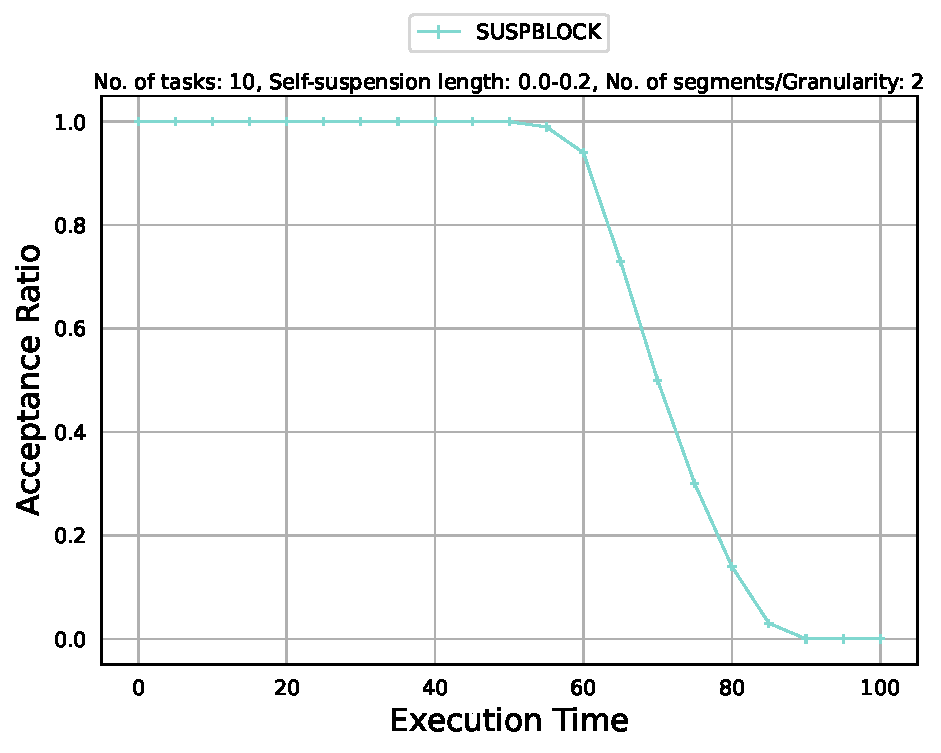
\includegraphics[width=\linewidth]{SUSPBLOCK[2][0.0-0.2][10].pdf}
		First UUnifast setup.
		\vspace{0.3cm}
		
		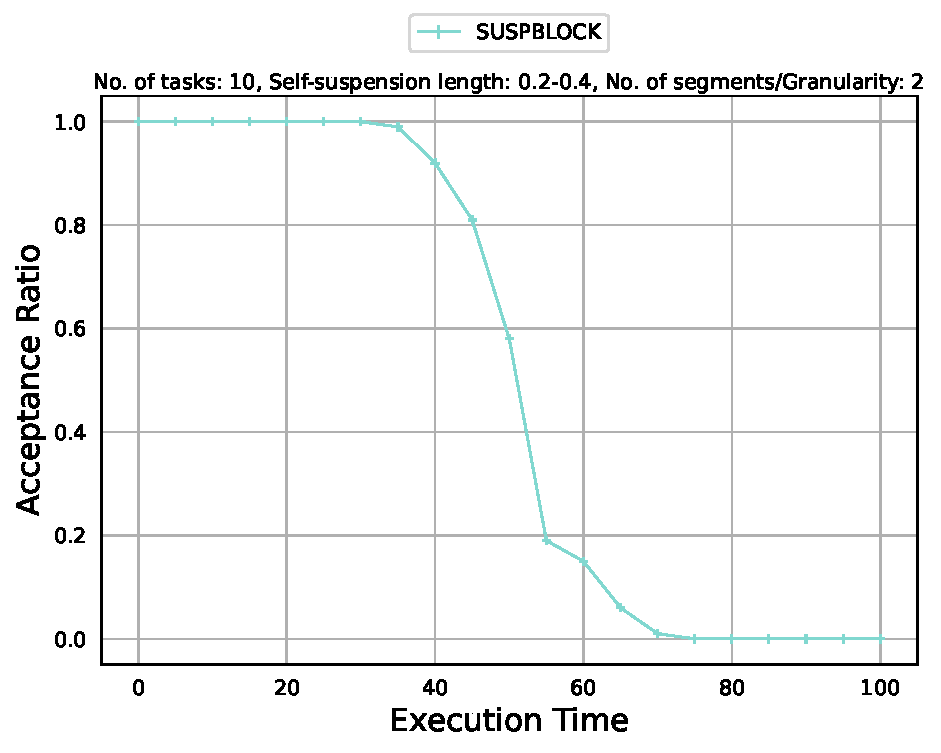
\includegraphics[width=\linewidth]{SUSPBLOCK[2][0.2-0.4][10].pdf}
		Second UUnifast setup.
		\vspace{0.3cm}
		
		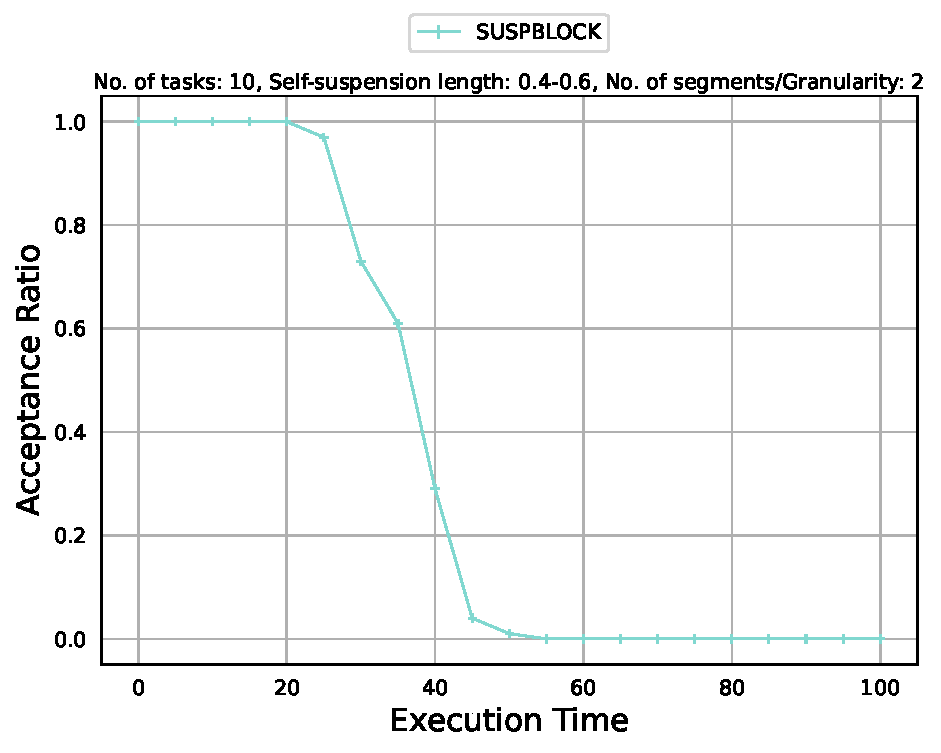
\includegraphics[width=\linewidth]{SUSPBLOCK[2][0.4-0.6][10].pdf}
		Third UUnifast setup.
		\vspace{0.3cm}
		
		
	\end{minipage}\hfill
	\begin{minipage}[t]{0.48\linewidth}
		\centering
		\textbf{(DRS)}
		\vspace{0.3cm}
		
		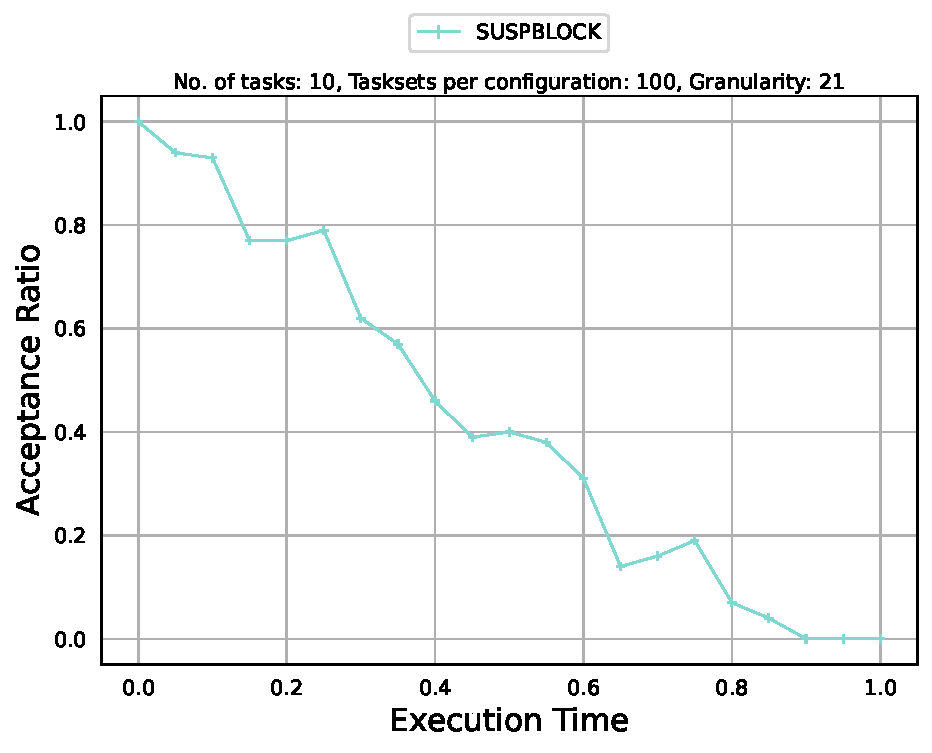
\includegraphics[width=\linewidth]{SUSPBLOCK_1stSetup_DRS.pdf}
		First DRS setup.
		\vspace{0.3cm}
		
		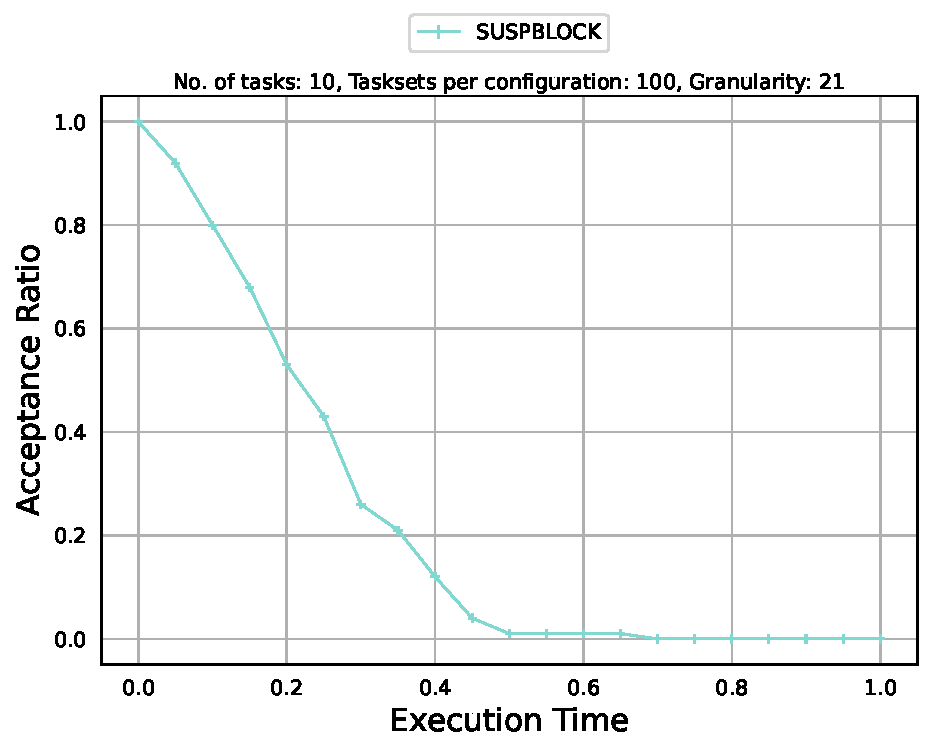
\includegraphics[width=\linewidth]{SUSPBLOCK_2ndSetup_DRS.pdf}
		Second DRS setup.
		\vspace{0.3cm}
		
		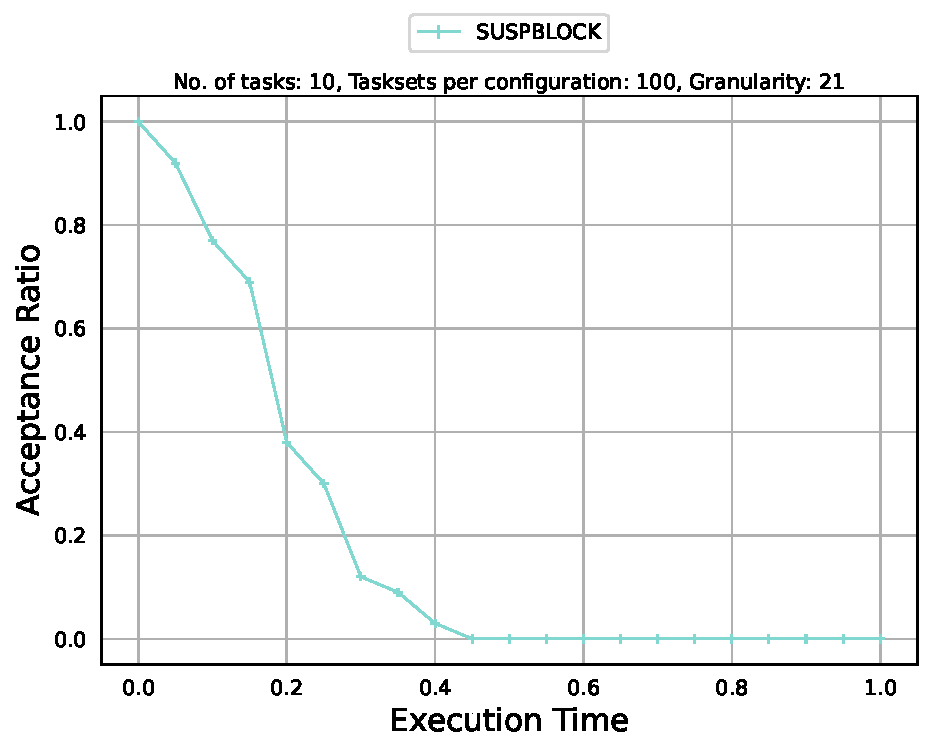
\includegraphics[width=\linewidth]{SUSPBLOCK_3rdSetup_DRS.pdf}
		Third DRS setup.
		\vspace{0.3cm}
	\end{minipage}


% ======================
	\clearpage
	\section{Idv Burst RM}
{
\raggedleft We are going to generate a Idv Burst RM schedule for the DRS and UUniFast setups explained above \newline 
}


	\begin{minipage}[t]{0.48\linewidth}
		\centering
		\textbf{(UUnifast)}
		\vspace{0.3cm}
		
		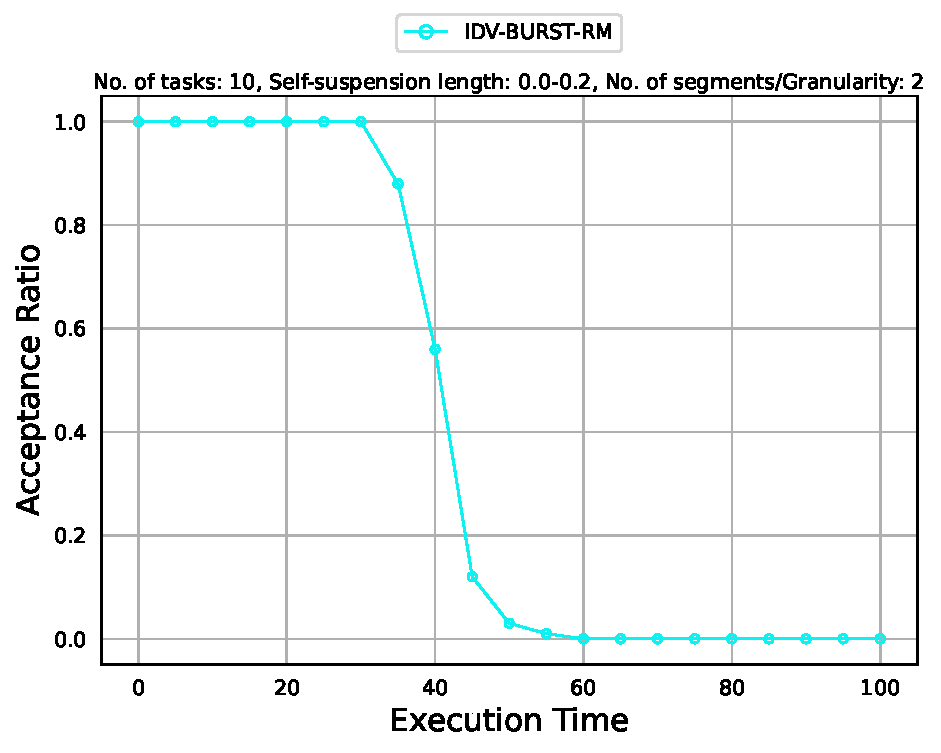
\includegraphics[width=\linewidth]{IDV-BURST-RM[2][0.0-0.2][10].pdf}
		First UUnifast setup.
		\vspace{0.3cm}
		
		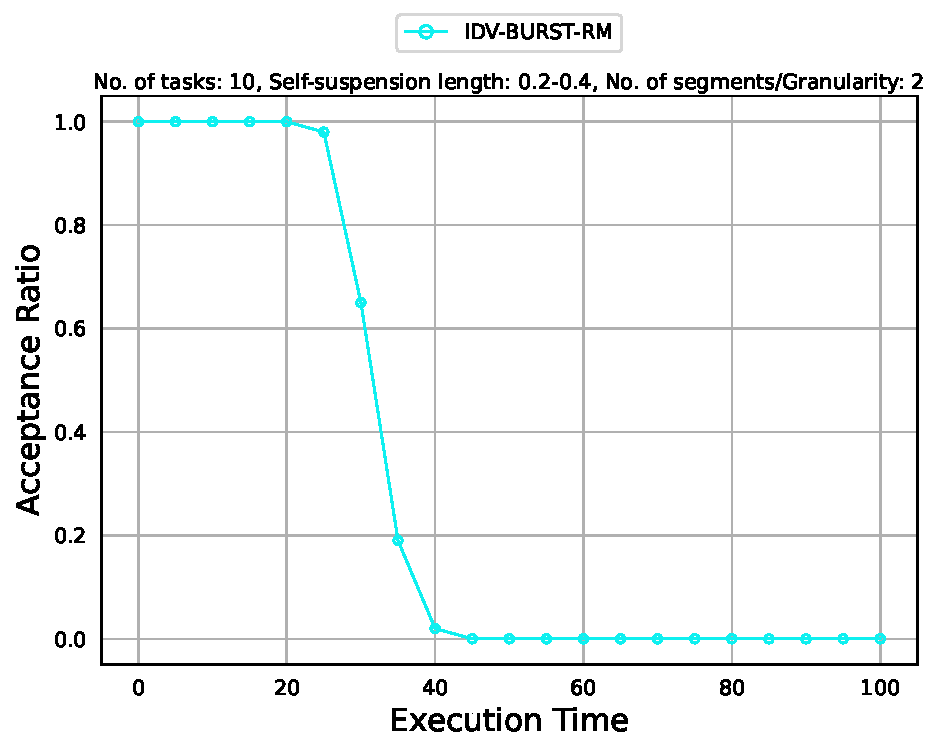
\includegraphics[width=\linewidth]{IDV-BURST-RM[2][0.2-0.4][10].pdf}
		Second UUnifast setup.
		\vspace{0.3cm}
		
		\includegraphics[width=\linewidth]{IDV-BURST-RM[2][0.4-0.6][10].pdf}
		Third UUnifast setup.
		\vspace{0.3cm}
		
		
	\end{minipage}\hfill
	\begin{minipage}[t]{0.48\linewidth}
		\centering
		\textbf{(DRS)}
		\vspace{0.3cm}
		
		\includegraphics[width=\linewidth]{IDV-BURST-RM_1stSetup_DRS.pdf}
		First DRS setup.
		\vspace{0.3cm}
		
		\includegraphics[width=\linewidth]{IDV-BURST-RM_2ndSetup_DRS.pdf}
		Second DRS setup.
		\vspace{0.3cm}
		
		\includegraphics[width=\linewidth]{IDV-BURST-RM_3rdSetup_DRS.pdf}
		Third DRS setup.
		\vspace{0.3cm}
	\end{minipage}

% ======================
	\clearpage
	\section{Comparing all tests at a glance}
{
\raggedleft We are comparing the all the different schedulability tests for both DRS and UUnifast for each of the setups \newline
}

	\begin{minipage}[t]{0.48\linewidth}
		\centering
		\textbf{(UUnifast)}
		\vspace{0.3cm}
		
		\includegraphics[width=\linewidth]{comparison_1stSetups_uni.pdf}
		First UUnifast setup.
		\vspace{0.3cm}
		
		\includegraphics[width=\linewidth]{comparison_2ndSetups_uni.pdf}
		Second UUnifast setup.
		\vspace{0.3cm}
		

		
	\end{minipage}\hfill
	\begin{minipage}[t]{0.48\linewidth}
		\centering
		\textbf{(DRS)}
		\vspace{0.3cm}
		
		\includegraphics[width=\linewidth]{comaprison_1stSetup_DRS.pdf}
		First DRS setup.
		\vspace{0.3cm}
		
		\includegraphics[width=\linewidth]{comaprison_2ndSetup_DRS.pdf}
		Second DRS setup.
		\vspace{0.3cm}

                   

	\end{minipage}



% ======================
        \clearpage
        
	\begin{minipage}[t]{0.48\linewidth}
		\centering
			
		\includegraphics[width=\linewidth]{comparison_3rdSetups_uni.pdf}
		Third UUnifast setup.
		\vspace{0.3cm}
		
		
	\end{minipage}\hfill
	\begin{minipage}[t]{0.48\linewidth}
		\centering
		
                   
		\includegraphics[width=\linewidth]{comaprison_3rdSetup_DRS.pdf}
		Third DRS setup.
		\vspace{0.3cm}
	\end{minipage}
% ======================
        \clearpage

        \section{SCEDF}
{
\raggedleft We are comparing the all the different schedulability tests for both DRS and UUnifast for each of the setups \newline
}

	\begin{minipage}[t]{0.48\linewidth}
		\centering
		\textbf{(UUnifast)}
		\vspace{0.3cm}
		
		\includegraphics[width=\linewidth]{SCEDF[2][0.0-0.02][10].pdf}
		First UUnifast setup.
		\vspace{0.3cm}
		
		\includegraphics[width=\linewidth]{SCEDF[2][0.02-0.04][10].pdf}
		Second UUnifast setup.
		\vspace{0.3cm}
		
            \includegraphics[width=\linewidth]{SCEDF[2][0.04-0.06][10].pdf}
		Third UUnifast setup.
		\vspace{0.3cm}
		
	\end{minipage}\hfill
	\begin{minipage}[t]{0.48\linewidth}
		\centering
		\textbf{(DRS)}
		\vspace{0.3cm}
		
		\includegraphics[width=\linewidth]{SCEDF_1st Setup.pdf}
		First DRS setup.
		\vspace{0.3cm}
		
		\includegraphics[width=\linewidth]{SCEDF_2nd Setup.pdf}
		Second DRS setup.
		\vspace{0.3cm}

            \includegraphics[width=\linewidth]{SCEDF_3rd Setup.pdf}
		Third DRS setup.
		\vspace{0.3cm}


                   

	\end{minipage}

% ======================
        \clearpage

        \section{SCRM}
{
\raggedleft We are comparing the all the different schedulability tests for both DRS and UUnifast for each of the setups \newline
}

	\begin{minipage}[t]{0.48\linewidth}
		\centering
		\textbf{(UUnifast)}
		\vspace{0.3cm}
		
		\includegraphics[width=\linewidth]{SCRM[2][0.0-0.02][10].pdf}
		First UUnifast setup.
		\vspace{0.3cm}
		
		\includegraphics[width=\linewidth]{SCRM[2][0.02-0.04][10].pdf}
		Second UUnifast setup.
		\vspace{0.3cm}
		
            \includegraphics[width=\linewidth]{SCRM[2][0.04-0.06][10].pdf}
		Third UUnifast setup.
		\vspace{0.3cm}
		
	\end{minipage}\hfill
	\begin{minipage}[t]{0.48\linewidth}
		\centering
		\textbf{(DRS)}
		\vspace{0.3cm}
		
		\includegraphics[width=\linewidth]{SCRM_1st Setup.pdf}
		First DRS setup.
		\vspace{0.3cm}
		
		\includegraphics[width=\linewidth]{SCRM_2nd Setup.pdf}
		Second DRS setup.
		\vspace{0.3cm}

            \includegraphics[width=\linewidth]{SCRM_3rd Setup.pdf}
		Third DRS setup.
		\vspace{0.3cm}


                   

	\end{minipage}

        
        

        
\section*{Evaluation:}      

{
\raggedleft \newline

So, the parameter we use to compare is \textbf{Acceptance Ratio} with respect to the execution time i.e the percentage of tasksets that got accepted for a particular execution time. We are generating 100 task sets per configuration with 10 tasks per set with a suspension values ranging between 0,0 - 0,6. \newline
}

\end{document}
